%---------------------------------------------------------------------------------
%                西南交通大学研究生学位论文：第五章内容
%---------------------------------------------------------------------------------
\chapter{系统设计与实现}\label{chap:system_implementation}

\section{引言}

第三章围绕政务智能问数中的可靠取数问题，提出了基于逻辑增强与异构协同的政务数据查询生成方法，重点解决自然语言问题到可执行SQL语句的准确映射问题；第四章进一步围绕分析规划、查询增强和轻量分析算子，提出了面向趋势、对比、排名和结构分析的数据分析方法，重点解决“查到数据之后如何开展规范分析”的问题。
然而，从论文方法到可交互原型之间仍然存在一层工程落地鸿沟：前端请求如何进入系统、查询与分析能力如何统一调度、上下文如何跨轮次继承、结果与日志如何沉淀并支持追溯，这些内容均需要在系统实现层面给出完整答案。

基于此，本章以“论文原型系统”为实现口径，将第三章的查询生成方法与第四章的分析生成方法整合为一个面向政务场景的智能问数原型系统。
本章不假设仓库外存在完整的互联网产品代码或复杂生产部署，而是围绕论文本身已验证的方法链路，说明一个真实可实现的原型系统如何完成从自然语言输入、可靠取数、结构化分析到结果组织与追溯的完整工程闭环。

从系统目标看，本章强调如下两类要求。

\textbf{功能目标}主要包括：
\textbf{（1）自然语言问数。} 支持用户以自然语言发起查询类或分析类任务，并自动进入相应处理链路；
\textbf{（2）可靠查询生成。} 复用第三章的LA-Schema增强、异构候选生成、查询修复与候选判别能力，输出高可信度SQL及其结果表；
\textbf{（3）自动化分析生成。} 复用第四章的AP-Schema构建、查询增强取数和分析算子编排能力，生成图表、表格与文字洞察；
\textbf{（4）结果留痕与追溯。} 完整保存任务状态、中间产物、执行日志和结果文件，以支持后续复核、复现与问题定位。

\textbf{非功能目标}则聚焦于工程可落地性：
\textbf{（1）可解释性。} 系统关键中间对象如LA-Schema、AP-Schema、最终SQL和结果包均可被查看与回溯；
\textbf{（2）可追溯性。} 每个任务的输入、执行路径与输出产物均有持久化记录；
\textbf{（3）可扩展性。} 查询服务、分析服务、上下文管理与数据存储相互解耦，便于后续扩展新的数据源与分析能力；
\textbf{（4）可控性。} 系统将查询与分析流程拆解为职责清晰的可管理模块，避免端到端黑盒生成带来的不可控问题。

围绕上述目标，本章从系统总体架构设计、业务流程设计、数据存储设计、多智能体协同与上下文管理实现以及系统功能展示五个方面展开，重点回答“第三章与第四章的方法如何被组织为统一原型系统”这一核心问题。


\section{系统总体架构设计}

为承接第三章与第四章的方法链路，并同时满足查询、分析、会话管理和结果追溯等工程需求，本文将原型系统设计为由表示层、应用层、智能服务层和数据层组成的四层架构，如图\ref{fig:chap05_architecture}所示。
这种分层方式使交互界面、任务调度、智能推理与底层数据管理彼此分离，从而避免将全部逻辑挤压到单一模块中，有利于保持系统结构清晰、职责稳定和后续演进能力。

\begin{figure}[htbp]
	\centering
	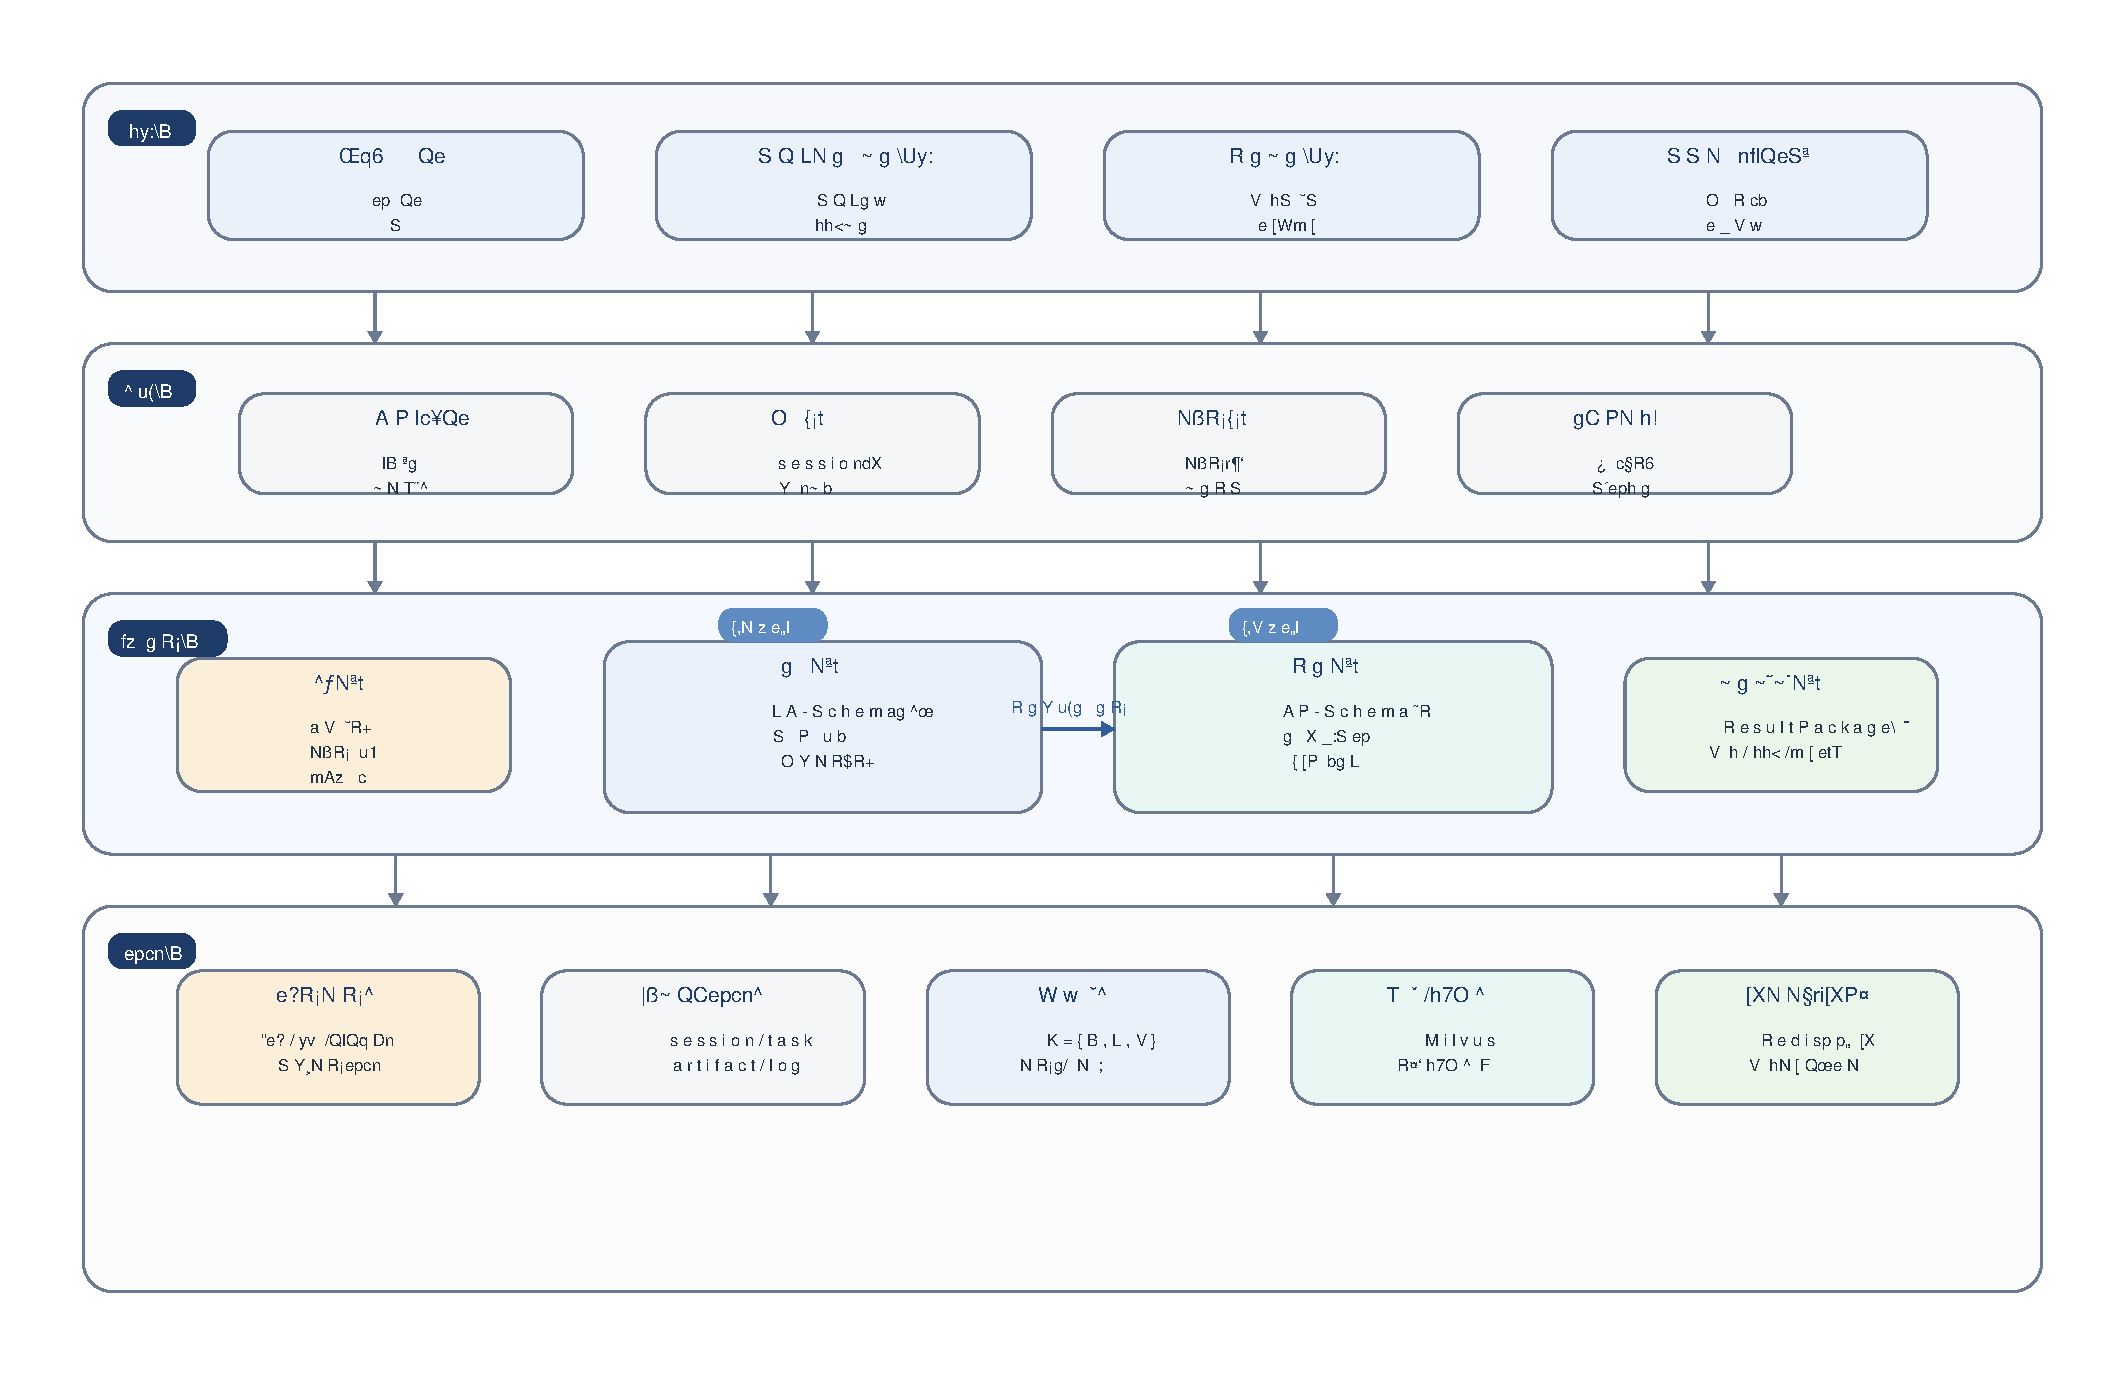
\includegraphics[width=0.98\textwidth]{figures/chap05/fig5-1_system_architecture.pdf}
	\caption{系统总体分层架构图}\label{fig:chap05_architecture}
\end{figure}

在该架构中，\textbf{表示层}直接面向用户，负责承接自然语言输入、呈现SQL与查询结果、展示分析图表与文字洞察，并提供历史会话与结果追溯入口。
表示层不直接承载方法逻辑，而是作为原型系统的人机交互界面，将用户请求组织为标准输入，并将下层返回的结构化结果可视化呈现。

\textbf{应用层}承担统一接入与会话管理职责。
其核心任务包括：接收前端请求并完成基础校验，维护用户会话与任务状态，将历史问题摘要、最近一次查询结果摘要等上下文注入下游服务，以及将执行结果统一回传给前端。
由于论文原型系统不以复杂企业级权限平台为目标，本层中的“权限与校验”主要体现为数据访问范围控制、参数合法性检查和任务状态一致性维护。

\textbf{智能服务层}是系统的核心。
其中，查询代理完整封装了第三章提出的方法链路，内部依次调用模式链接（\ref{subsec:schema_linking}节）、异构候选生成（\ref{subsec:candidate_generation}节）、查询修复（\ref{subsec:query_repair}节）和候选判别（\ref{subsec:candidate_selection}节），对外表现为稳定的查询生成服务；
分析代理则封装第四章的分析规划与结果生成能力，内部依次调用AP-Schema构建（\ref{subsec:ap_schema_build}节）、查询需求投影（\ref{subsec:task_partition}节）、轻量分析算子编排（\ref{subsec:operator_orchestration}节）和结果生成（\ref{subsec:result_pipeline}节），对外表现为分析生成服务；
调度代理负责意图识别、任务路由和服务编排，结果组织代理负责将异构执行产物统一封装为面向前端与追溯的标准结果包。
特别地，分析代理在取数阶段并不自行生成SQL，而是通过标准接口复用查询代理，从而实现“先查准、再分析”的层级协同。

\textbf{数据层}为上层服务提供稳定的数据与知识支撑。
一方面，政务业务库保存财政、项目、公共资源等原始数据，是查询与分析的最终数据来源；
另一方面，系统元数据库、领域知识库、向量库与样例库、缓存和结果文件存储共同构成系统运行所需的工程底座。
其中，领域知识库直接承接第三章\ref{subsec:knowledge_base_construction}节中构建的$K=\{B,L,V\}$，动态样例库承接第三章\ref{subsec:dynamic_example_retrieval}节中构建的$F$，二者共同参与在线查询链路；系统元数据库则为任务状态管理、产物登记和会话上下文维护提供持久化支撑。

系统核心模块及其职责如表\ref{tab:chap05_modules}所示。

\begin{table}[htbp]
	\setlength{\abovecaptionskip}{5pt}
	\setlength{\belowcaptionskip}{5pt}
	\caption{系统核心模块及职责说明}\label{tab:chap05_modules}
	\centering
	\footnotesize
	\renewcommand{\arraystretch}{1.3}
	\begin{tabular}{p{2.1cm}p{3.8cm}p{7.2cm}}
		\toprule
		层次 & 核心模块 & 主要职责 \\
		\midrule
		表示层 & 自然语言输入、结果展示、历史追溯入口 & 接收问数请求，展示SQL、结果表、图表、洞察和任务日志，支持历史会话切换与追问。 \\
		应用层 & API接入、会话管理、任务管理、请求校验 & 组织标准请求参数，维护\texttt{session\_summary}与任务状态，向智能服务层分发任务并统一回传结果。 \\
		智能服务层 & 调度代理 & 识别请求属于查询还是分析任务，执行路由、编排与结果汇总。 \\
		智能服务层 & 查询代理 & 封装第三章查询生成方法，输出\texttt{final\_sql}、\texttt{result\_table}、执行状态和查询日志。 \\
		智能服务层 & 分析代理 & 封装第四章分析规划与分析算子方法，复用查询代理完成查询增强取数并生成分析结果。 \\
		智能服务层 & 结果组织代理 & 将图、表、文和日志统一封装为\texttt{ResultPackage}，供前端展示与结果追溯。 \\
		数据层 & 政务业务库、系统元数据库、知识与检索存储 & 保存原始业务数据、系统状态、领域知识、向量检索索引、样例索引、缓存与结果文件。 \\
		\bottomrule
	\end{tabular}
	\renewcommand{\arraystretch}{1.0}
\end{table}

综上，本系统并不是在第三章与第四章之外再构建一套新的问数逻辑，而是将“查询生成服务”和“分析生成服务”组织到统一的分层架构中。
前者负责把自然语言可靠地映射为标准取数结果，后者负责在可靠数据基础上完成规范化分析，二者经由调度代理和共享上下文共同组成论文原型系统的核心处理链。


\section{业务流程设计}

系统总体架构回答了“模块如何组织”的问题，而业务流程进一步回答“请求如何流动”的问题。
对本研究提出的政务智能问数原型而言，系统既要支持面向数据库的直接查询，也要支持基于查询结果的分析任务，并在任一关键节点发生异常时能够终止、修复或追溯。
因此，本节分别从智能查询流程、智能分析流程以及异常回退与结果追溯流程三个方面展开说明。

\begin{figure}[htbp]
	\centering
	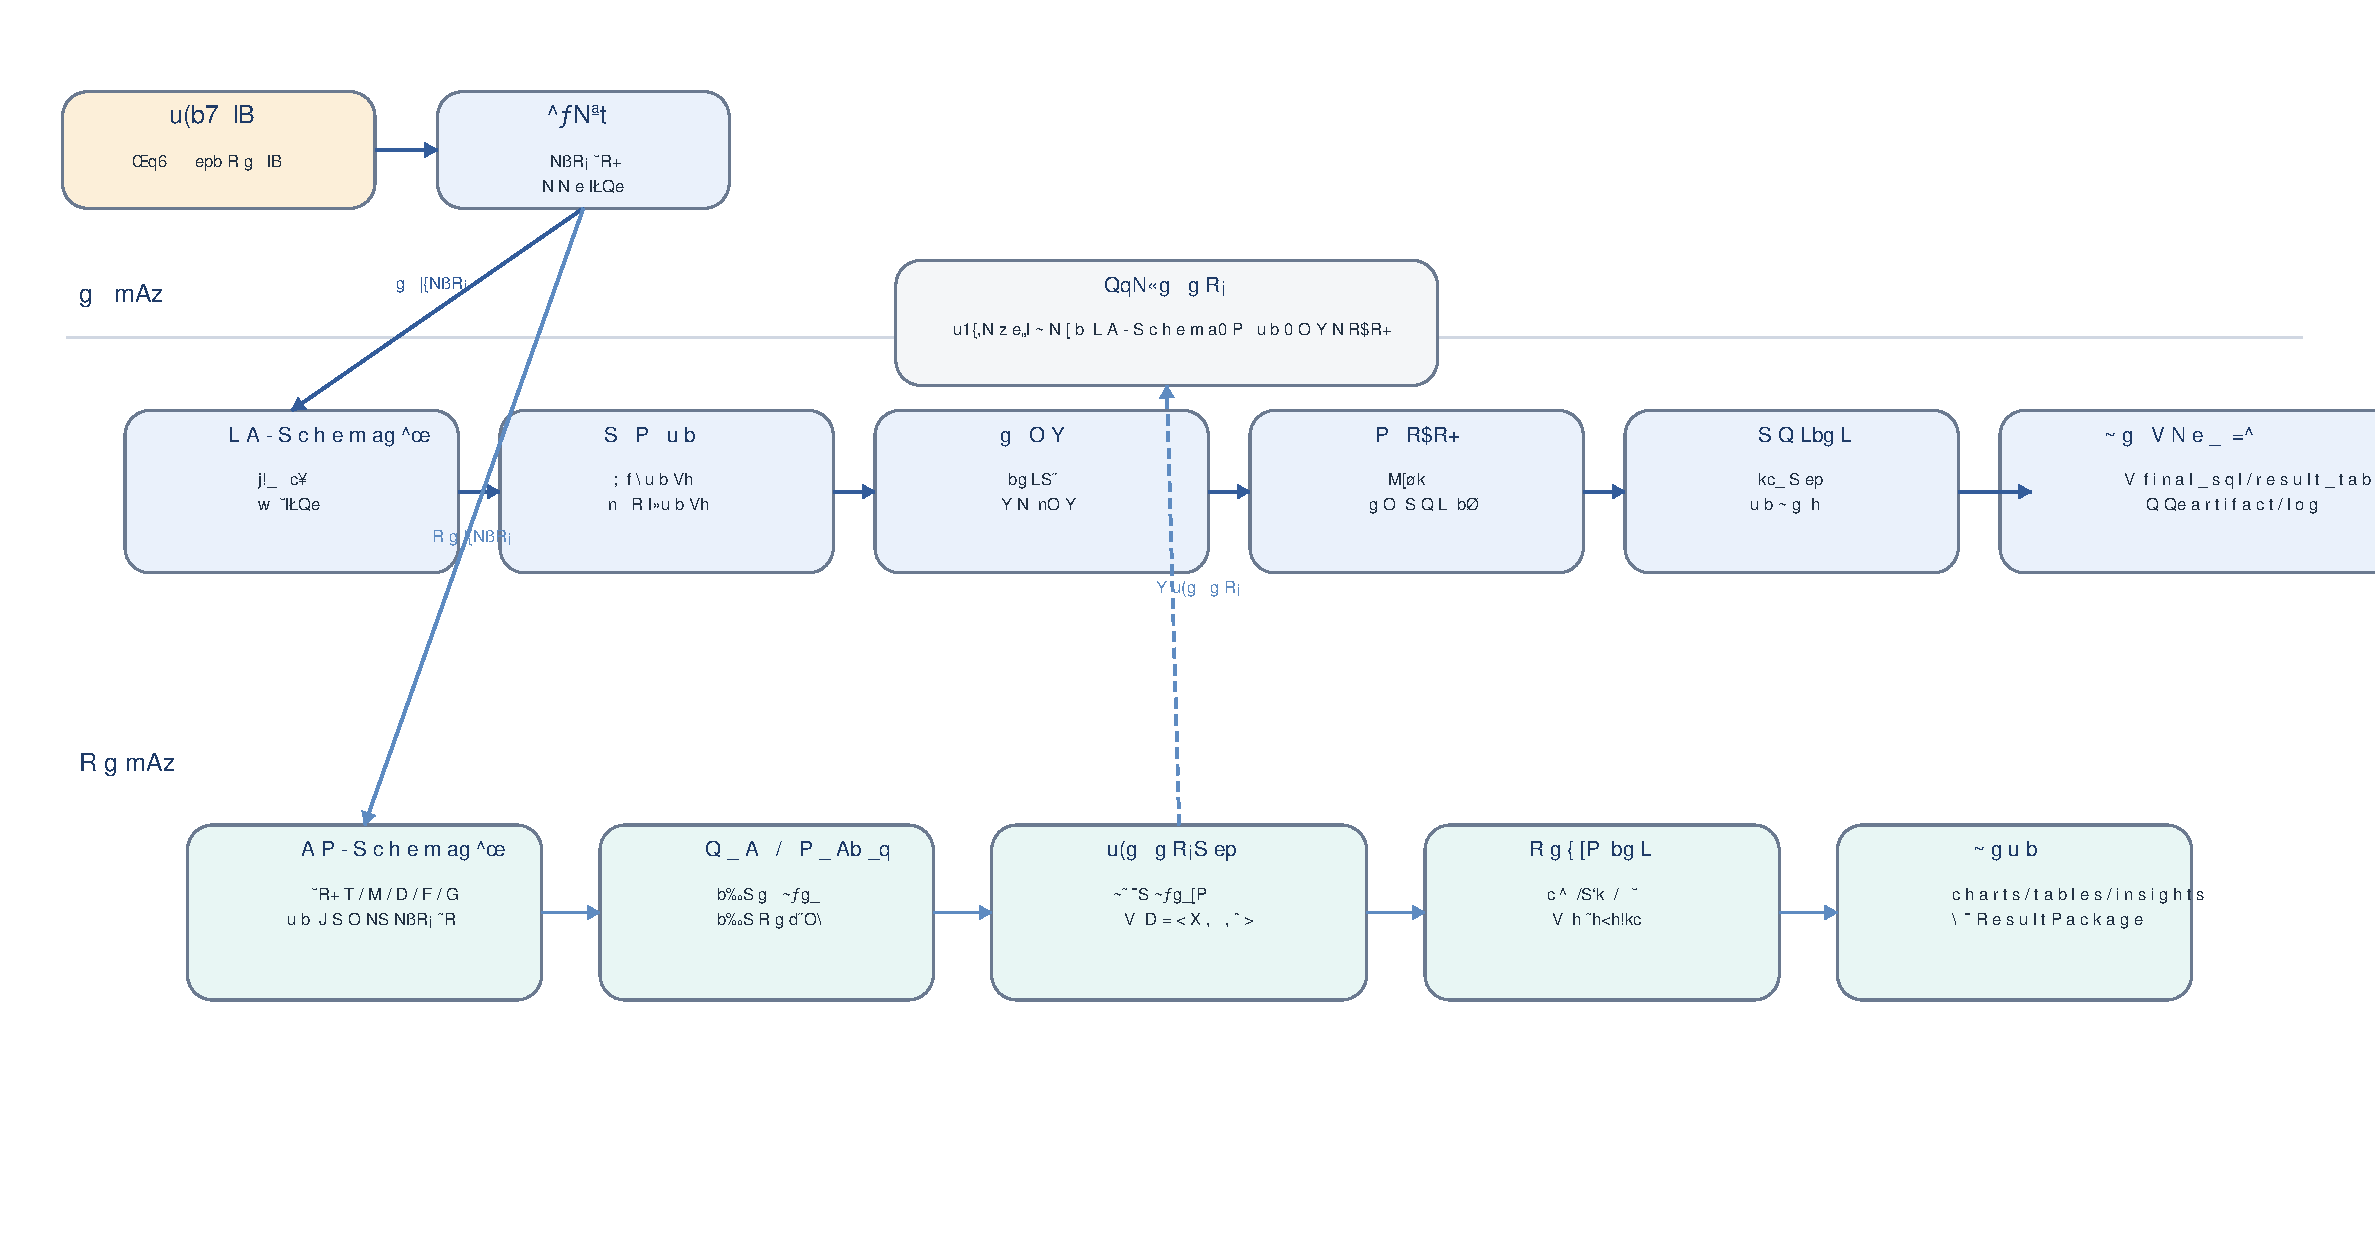
\includegraphics[width=1.0\textwidth]{figures/chap05/fig5-2_dual_workflow.pdf}
	\caption{智能查询与智能分析双流程图}\label{fig:chap05_dual_workflow}
\end{figure}

\subsection{智能查询业务流程}

如图\ref{fig:chap05_dual_workflow}上半部分所示，当调度代理识别到用户输入属于查询类任务时，系统启动完整的查询生成链路，其执行过程与第三章的方法一一对应，但在工程实现上被组织为以下顺序明确的步骤。

\textbf{步骤1：任务识别与上下文注入。}
应用层首先接收自然语言请求，并从当前会话中读取最近的历史问题摘要、上一次成功查询的\texttt{final\_sql}、最近一次结果表摘要以及用户在上文中已经明确指定的约束条件。
这些信息被压缩组织为\texttt{session\_summary}，与当前\texttt{nl\_query}共同构成查询服务输入，从而支撑连续追问和省略式表达的解析。

\textbf{步骤2：LA-Schema构建。}
查询代理接收到请求后，进入第三章定义的模式链接阶段。
系统先读取业务数据源对应的表结构、字段注释、样例值和主外键关系，再结合领域知识库中的业务术语映射、逻辑计算规则和值域约束，构建当前问题对应的逻辑增强模式LA-Schema。
在工程上，LA-Schema不仅是模型提示的一部分，也会以\texttt{la\_schema\_snapshot}形式写入元数据库，便于后续排错和结果复核。

\textbf{步骤3：双路候选生成。}
在得到LA-Schema后，系统并行调用逻辑映射生成器和渐进分治生成器。
前者优先利用业务术语映射和虚拟逻辑列快速生成标准查询，后者通过结构化推理链逐步生成复杂SQL。
二者共同产出多样化候选集，为后续判别提供更大的搜索覆盖面。

\textbf{步骤4：查询修复。}
系统对所有候选SQL执行预执行检查。
若出现语法错误、字段名错误、连接条件缺失或其他执行异常，则触发查询修复器；修复器结合原问题、LA-Schema和数据库错误信息进行有限轮次的反思修复。
当修复成功时，候选被保留并重新进入候选池；当修复达到上限仍失败时，候选被标记为不可用，同时将错误明细写入日志。

\textbf{步骤5：候选判别与最优SQL确定。}
在候选池质量得到提升后，系统调用第三章定义的候选判别模型，对执行结果不同的候选SQL进行配对比较，并通过得分聚合选出最优SQL。
此时，查询服务对外输出的核心对象包括最终SQL语句\texttt{final\_sql}、结果表\texttt{result\_table}、执行状态\texttt{execution\_status}、查询日志\texttt{logs}以及LA-Schema快照\texttt{la\_schema\_snapshot}。

\textbf{步骤6：正式执行与结果返回。}
最优SQL在目标政务业务库上正式执行后，结果表会被封装为结构化记录返回给应用层。
同时，系统将问题文本、最终SQL、执行状态、中间日志、结果表摘要以及相关产物统一写入系统元数据库。
因此，查询流程的最终结果不仅用于当前页面展示，也成为后续分析任务可复用的标准取数结果。

通过上述设计，第三章中的查询生成方法被工程化封装为可调用服务。
其中，输入侧由\texttt{nl\_query}、\texttt{session\_summary}和可选约束\texttt{optional\_constraints}构成；输出侧则统一返回\texttt{final\_sql}、\texttt{result\_table}、\texttt{execution\_status}、\texttt{logs}和\texttt{la\_schema\_snapshot}。
这一稳定接口也是分析服务能够复用查询服务的前提。

\subsection{智能分析业务流程}

如图\ref{fig:chap05_dual_workflow}下半部分所示，当调度代理判断用户需求属于趋势分析、对比分析、排名分析或结构分析时，系统进入分析生成链路。
该链路并非重新从自然语言直接生成一套新的SQL与图表，而是严格遵循第四章提出的“分析规划、查询增强、算子执行、结果组织”逻辑，其工程步骤如下。

\textbf{步骤1：分析意图识别与AP-Schema构建。}
分析代理首先解析原始需求中的分析类型、指标、维度、筛选条件、时间粒度和展示要求，并构建JSON化的任务规划对象\texttt{ap\_schema}。
该对象在系统中对应第四章的
\begin{equation}
\texttt{ap\_schema}=\{T,M,D,\hat{F},G,O_q,O_a,\hat{V},\hat{S}\},
\end{equation}
其中各字段分别对应分析类型、指标集合、维度集合、筛选条件、粒度、查询层操作、分析层操作、可视化规格和摘要要求。
在工程实现中，\texttt{ap\_schema}将被持久化保存到\texttt{analysis\_task}表中，并作为分析执行过程的主控对象。

\textbf{步骤2：查询投影与查询增强取数。}
分析代理从\texttt{ap\_schema}中进一步投影出查询需求$Q_A$与分析需求$P_A$。
其中，$Q_A$承载指标、维度、过滤条件、时间粒度和需在查询层完成的业务口径；$P_A$承载分析算子、可视化要求和摘要生成要求。
随后，分析代理将$Q_A$与原始自然语言需求重新组装为受约束查询子问题，并通过统一接口调用查询代理。
也就是说，分析服务在取数阶段并不直接生成SQL，而是将复杂业务口径继续交由第三章已经验证有效的查询链路求解。

\textbf{步骤3：标准查询结果接口返回。}
查询代理执行完上述受约束子问题后，向分析代理返回标准结果接口
\begin{equation}
\mathcal{D}=\langle \mathbf{X}, \Gamma, \sigma \rangle,
\end{equation}
其中$\mathbf{X}$表示查询结果数据表，$\Gamma$表示字段语义与元数据信息，$\sigma$表示执行状态。
这一接口在工程上具有两层意义：一是将“是否查到数据”的判断与“如何组织分析结果”的判断分开；二是使分析层只依赖标准输入，而不需要关心具体SQL如何生成。

\textbf{步骤4：分析算子链执行。}
当$\sigma=\text{success}$时，分析代理根据$P_A$中的$O_a$、$\hat{V}$和$\hat{S}$组织轻量分析算子链，对$\mathbf{X}$执行排序、占比计算、Top-K提取、透视和重点标注等操作，并根据字段类型和类别数对初始图表规格作后校正。
若$\sigma=\text{failure}$，则分析流程直接中止，并将查询失败信息写入分析日志，避免在无效数据上继续生成分析结论。

\textbf{步骤5：结果组织与标准输出。}
分析代理将图表、表格、文字洞察和执行日志统一交由结果组织代理封装为
\begin{equation}
\texttt{ResultPackage}=\{\texttt{charts},\texttt{tables},\texttt{insights},\texttt{logs}\},
\end{equation}
其中\texttt{charts}面向图表展示与导出，\texttt{tables}保存规整后的分析表，\texttt{insights}保存自动生成的结论摘要，\texttt{logs}记录执行过程和异常信息。
该结果包既是前端页面展示的直接输入，也是结果追溯和复用的统一产物格式。

为了更直观地展示一次分析任务在系统内部的端到端执行顺序，图\ref{fig:chap05_sequence}给出了分析请求从前端进入应用层，经调度代理、分析代理、查询代理、数据库和结果组织代理后再返回前端的完整时序关系。

\begin{figure}[htbp]
	\centering
	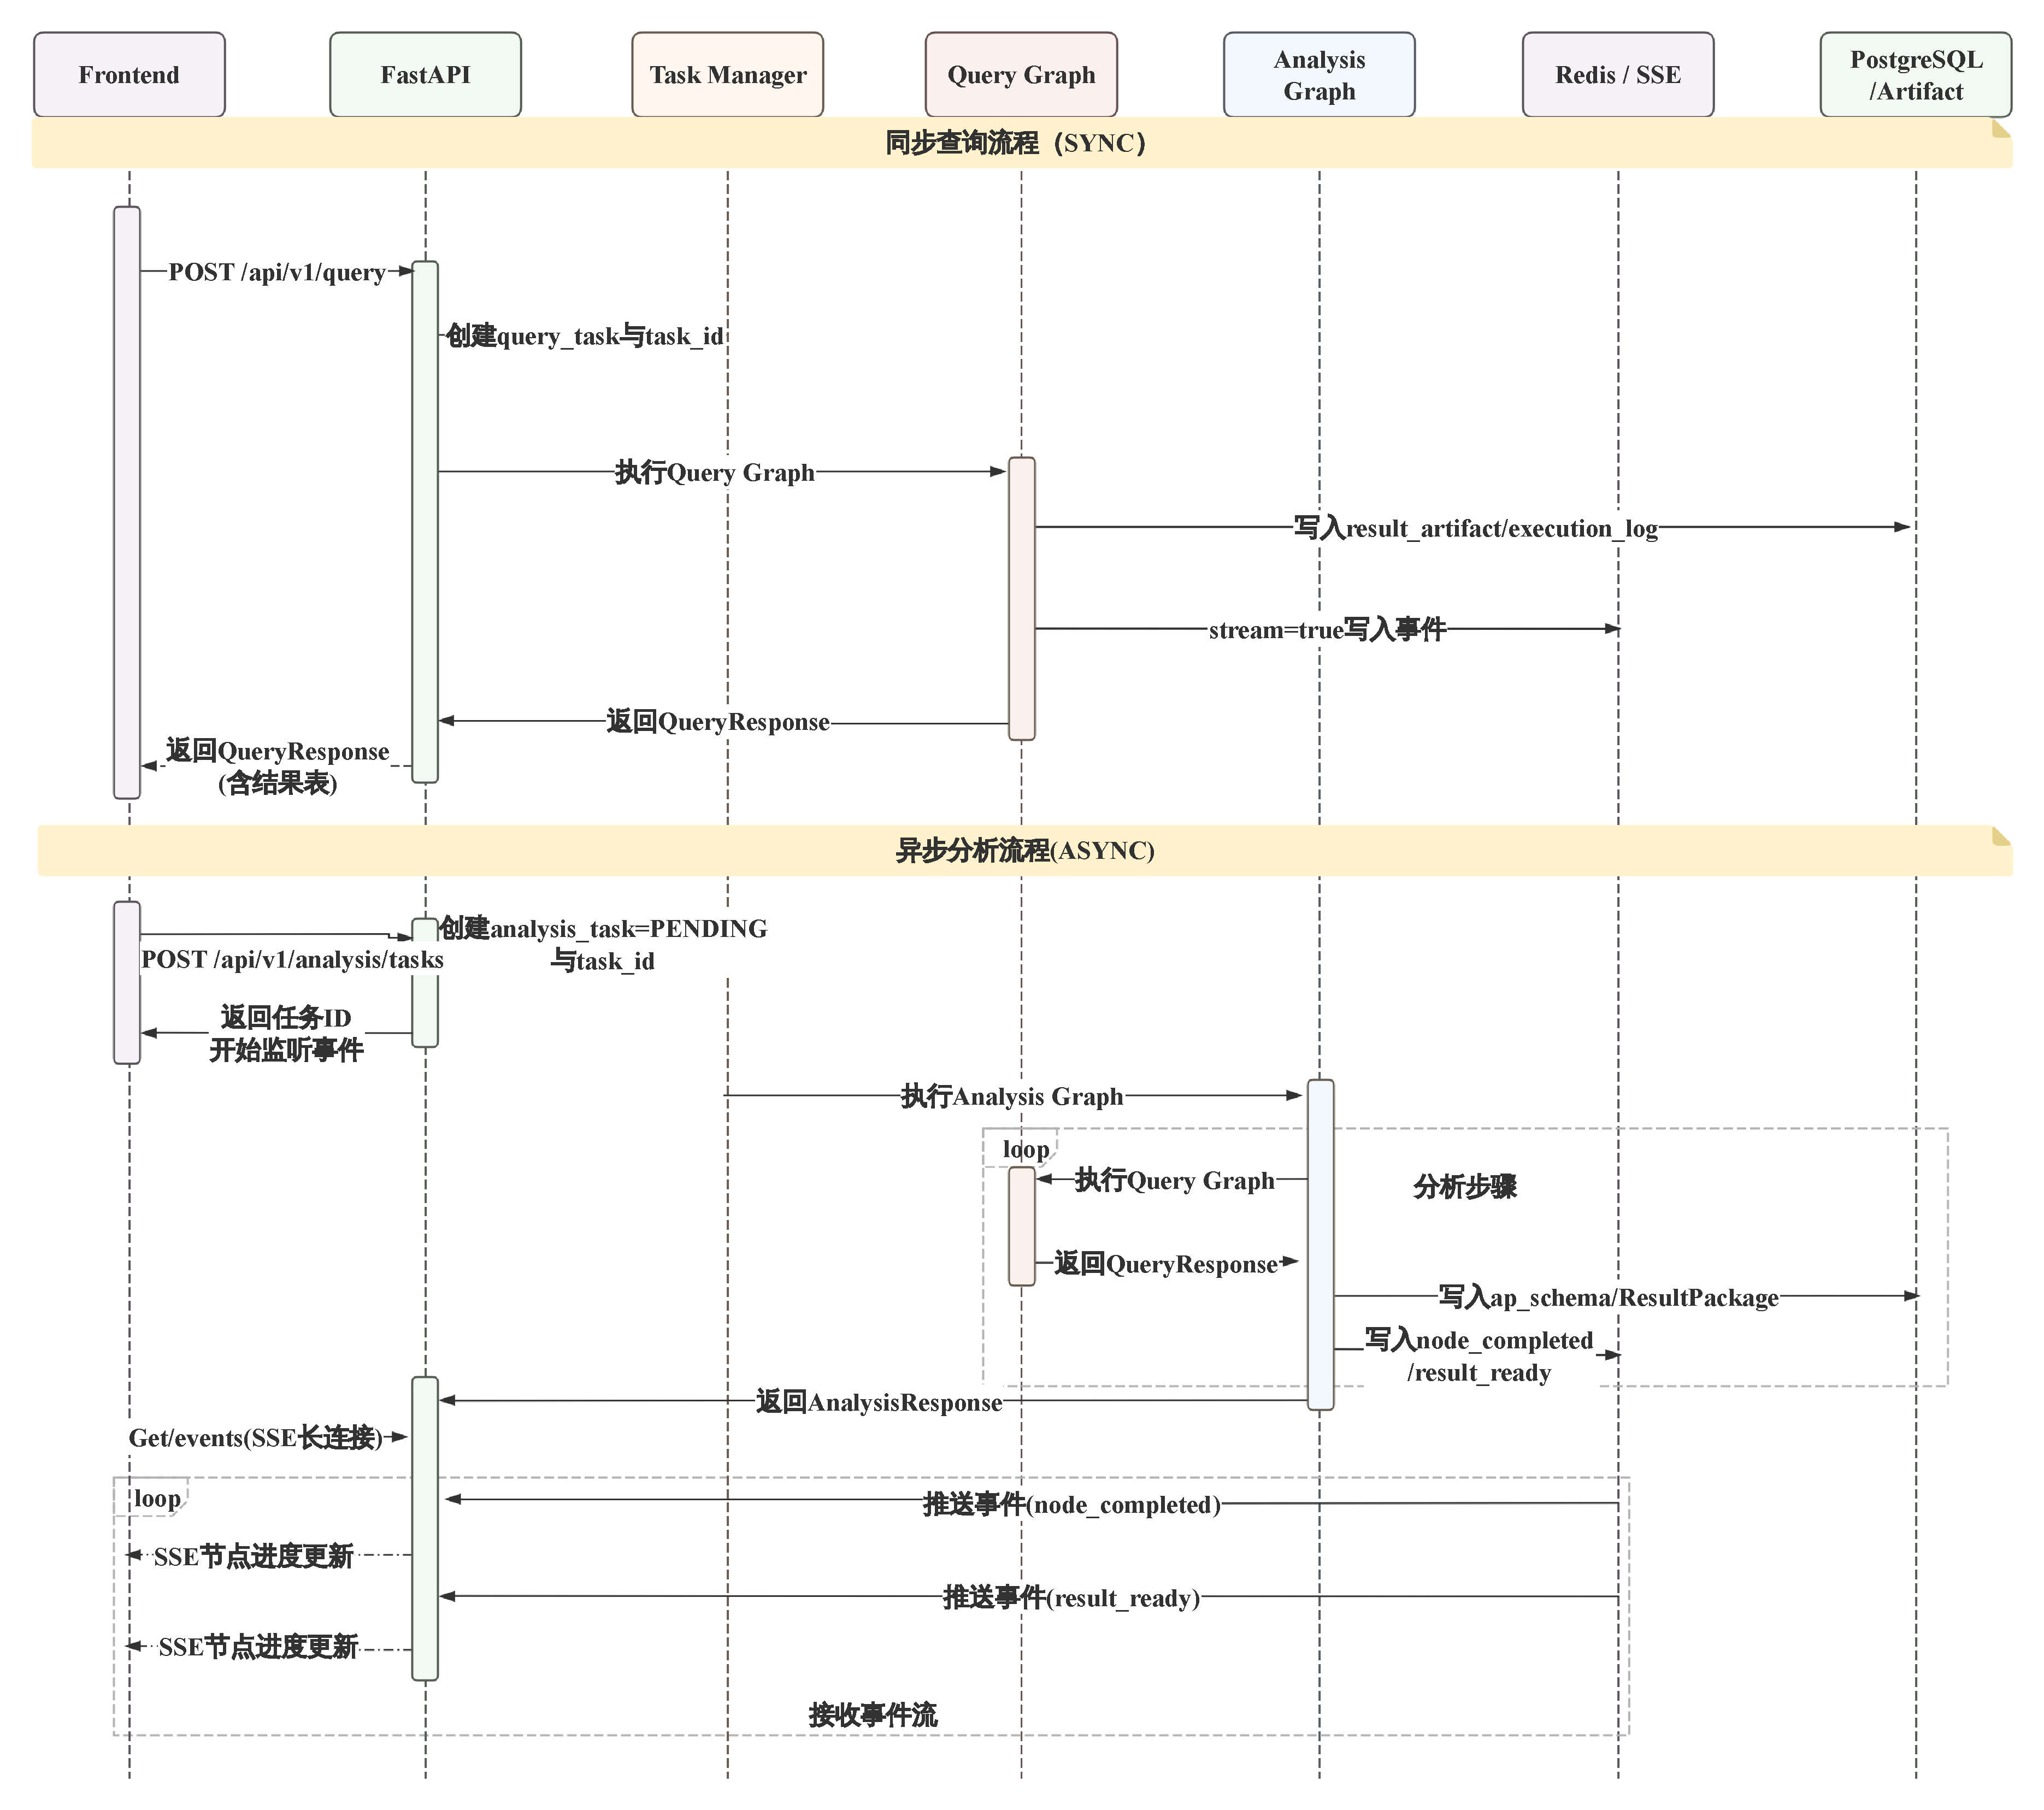
\includegraphics[width=1.0\textwidth]{figures/chap05/fig5-4_analysis_sequence.pdf}
	\caption{分析任务端到端时序图}\label{fig:chap05_sequence}
\end{figure}

\subsection{异常回退与结果追溯流程}

政务问数与分析场景对结果可靠性要求较高，因此系统不能仅在“成功路径”上工作，还必须能够处理查询失败、空结果、分析脚本异常和超时等异常情况。
为此，系统在查询服务和分析服务之外额外设计了异常回退与结果追溯机制，其流程如图\ref{fig:chap05_exception}所示。

\begin{figure}[htbp]
	\centering
	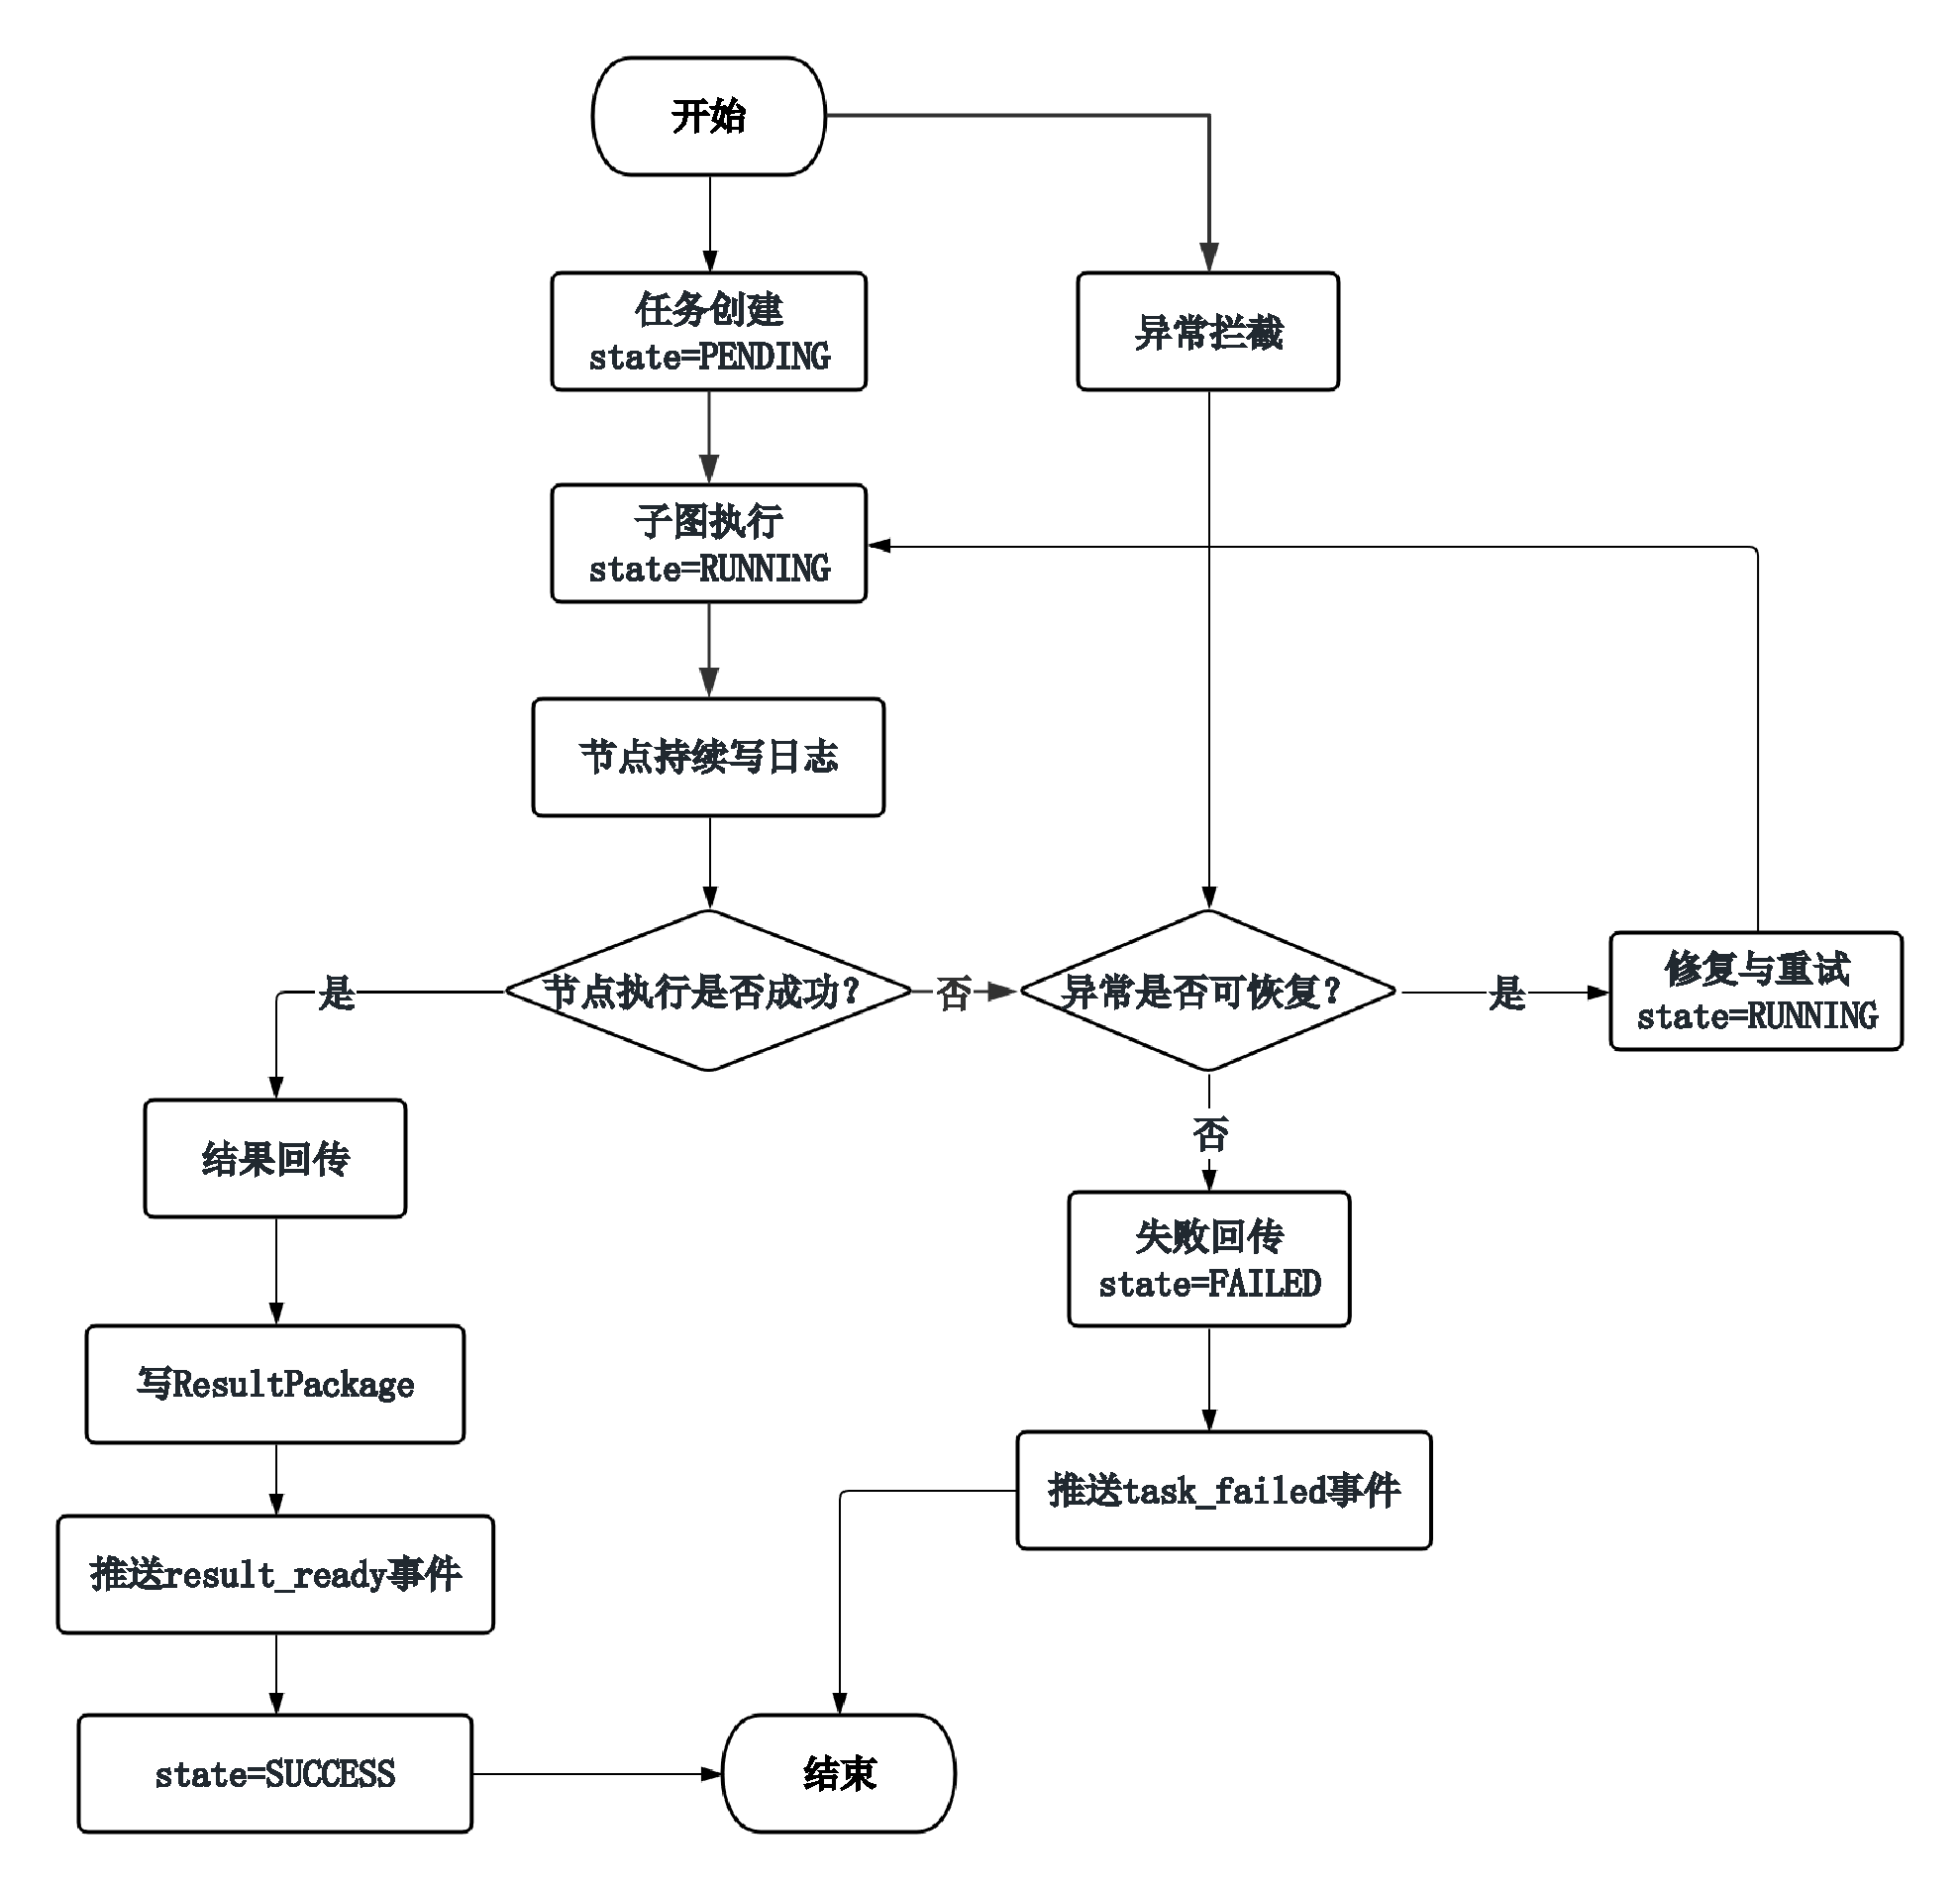
\includegraphics[width=0.95\textwidth]{figures/chap05/fig5-7_exception_trace.pdf}
	\caption{异常回退与结果追溯流程图}\label{fig:chap05_exception}
\end{figure}

具体而言，系统先根据失败发生的位置对异常进行分类。
若异常出现在查询阶段，则重点区分字段名错误、连接关系错误、值匹配错误和数据库执行超时等类型；若异常出现在分析阶段，则重点区分查询返回空结果、算子执行失败、图表映射不满足条件和结果封装异常等类型。
对于可恢复错误，系统优先采用有限轮次的自动修复与重试策略，例如调用查询修复器、调整查询参数或重新选择算子链；对于不可恢复错误，则立即终止流程并返回明确的失败说明，避免给用户输出误导性结论。

与此同时，系统将每个关键节点的状态变化和中间对象写入\texttt{execution\_log}与\texttt{result\_artifact}。
当用户需要查看“为什么这次分析失败”“最终SQL是如何得到的”或“当前图表对应的是哪一份结果表”时，系统可以按任务ID回溯到原始问题、LA-Schema快照、AP-Schema对象、最终SQL、标准查询结果接口$\mathcal{D}$、最终\texttt{ResultPackage}以及相关日志，从而形成完整的结果追溯链路。
这种设计保证了第五章所实现的原型系统并不是一个无法解释的黑盒，而是一个在关键节点上可以被审计和复核的工程系统。


\section{系统数据存储}

要让上述查询流程、分析流程和追溯机制稳定运行，仅有算法模块还不够，还需要有针对性的存储设计来承接数据源接入、元数据抽取、任务状态保存和结果产物管理。
因此，本节从业务数据源接入与元数据抽取、系统元数据库设计以及结果与缓存管理三个方面说明数据存储实现。

\subsection{业务数据源接入与元数据抽取}

本研究服务于真实政务数据环境，因此系统首先需要能够接入财政、项目、公共资源等不同部门的业务数据库。
在工程实现上，系统通过JDBC/ODBC等标准数据库连接方式建立到外部数据源的连接，并在\texttt{data\_source}表中维护数据源标识、数据库类型、连接配置和同步策略等元信息。

仅仅建立连接并不足以支撑第三章的模式链接和LA-Schema构建，系统还必须对外部数据源执行结构化元数据抽取。
如图\ref{fig:chap05_metadata}所示，元数据抽取流程包含表结构抽取、字段属性抽取、主外键关系抽取以及样例值和枚举值抽取四个环节。

\begin{figure}[htbp]
	\centering
	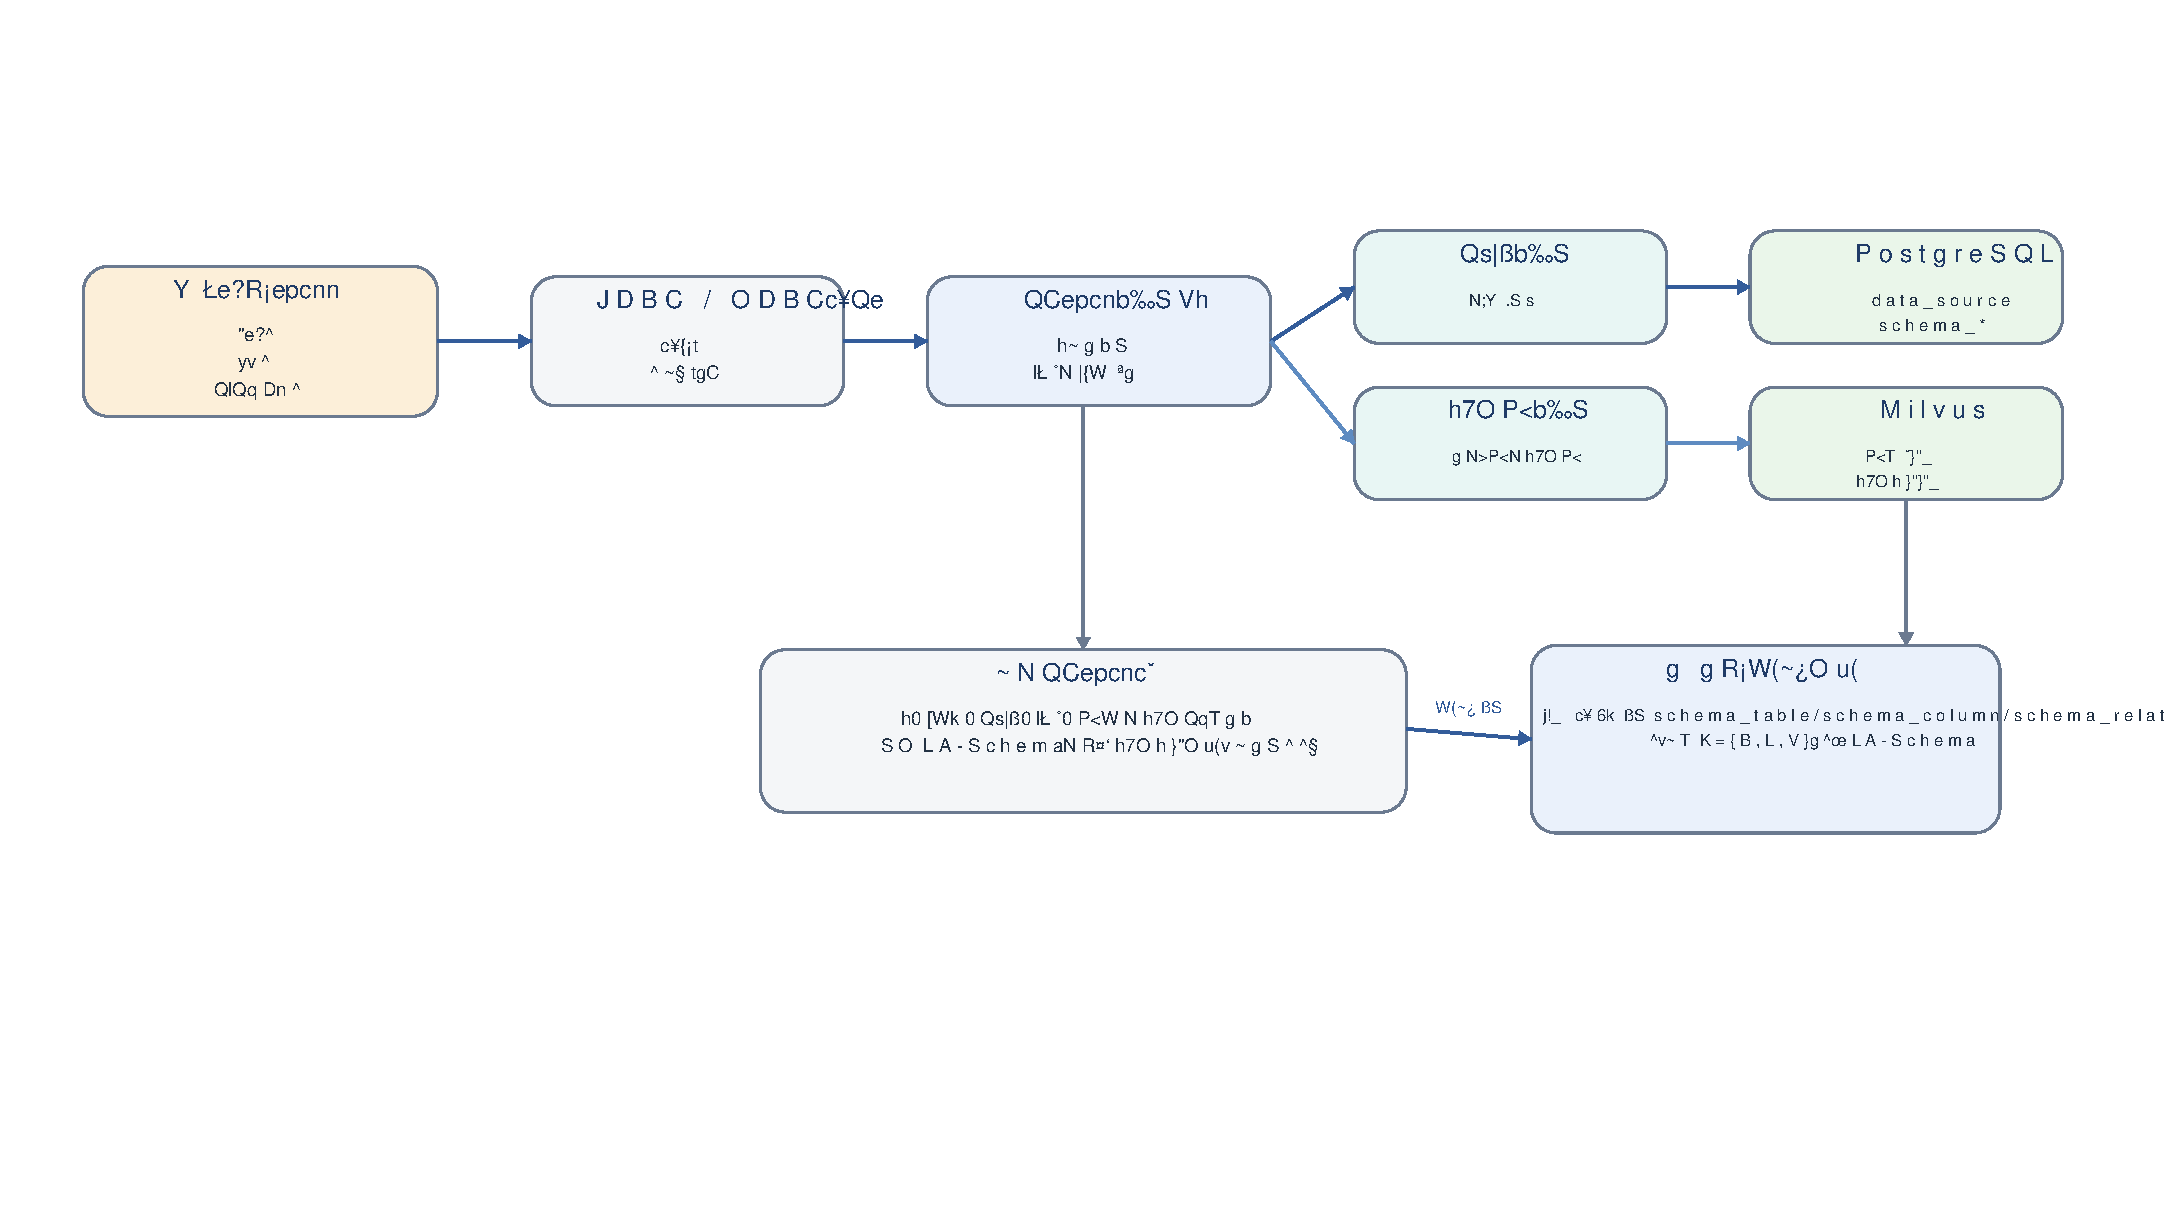
\includegraphics[width=0.98\textwidth]{figures/chap05/fig5-5_metadata_extraction.pdf}
	\caption{业务数据源接入与元数据抽取流程图}\label{fig:chap05_metadata}
\end{figure}

其中，\textbf{表结构抽取}负责获得库、表和字段的基础信息，包括表名、表注释、字段名、数据类型、主键标识和字段注释等；
\textbf{关系抽取}负责显式发现数据库中的主外键关系，并将其转化为统一的\texttt{schema\_relation}记录，以支撑后续多表JOIN推理；
\textbf{样例值抽取}面向行政区划、项目状态、支出类别等典型枚举型或文本型字段，抽取少量样例值或完整值域，用于值匹配与语义提示；
\textbf{向量索引构建}则将关键字段值与动态样例检索所需内容编码后写入Milvus，为第三章中的值检索与样例检索提供在线支持。

经过上述过程后，系统在PostgreSQL中形成\texttt{data\_source}、\texttt{schema\_table}、\texttt{schema\_column}和\texttt{schema\_relation}等标准元数据表，在Milvus中形成面向值检索与样例检索的向量索引。
在线查询时，查询代理会首先从这些元数据对象中读取与当前问题相关的结构信息，再与领域知识库$K=\{B,L,V\}$和动态样例库$F$共同构建LA-Schema。
因此，元数据抽取模块实际上承担了从“外部数据库原始结构”到“可被智能查询方法使用的统一知识表示”之间的桥梁作用。

\subsection{系统元数据库设计}

除了外部业务数据源之外，系统自身还需要一个独立的元数据库来持久化保存会话、任务、产物和日志等状态对象。
围绕这一目标，本文设计了如表\ref{tab:chap05_metadata_tables}所示的系统核心数据表，并在图\ref{fig:chap05_er}中给出了它们之间的主要关联关系。

\begin{table}[htbp]
	\setlength{\abovecaptionskip}{5pt}
	\setlength{\belowcaptionskip}{5pt}
	\caption{系统元数据库核心表设计}\label{tab:chap05_metadata_tables}
	\centering
	\scriptsize
	\renewcommand{\arraystretch}{1.25}
	\begin{tabular}{p{3.4cm}p{3.7cm}p{5.4cm}}
		\toprule
		表名 & 关键字段 & 主要说明 \\
		\midrule
		\texttt{data\_source} & \makecell[tl]{\texttt{source\_id}\\\texttt{source\_name}\\\texttt{db\_type}} & 保存外部政务数据源配置和同步信息，是元数据抽取的起点。 \\
		\texttt{schema\_table} & \makecell[tl]{\texttt{table\_id}\\\texttt{source\_id}\\\texttt{table\_name}} & 保存库级与表级结构信息，供模式链接和多库定位使用。 \\
		\texttt{schema\_column} & \makecell[tl]{\texttt{column\_id}\\\texttt{table\_id}\\\texttt{column\_name}\\\texttt{sample\_values}} & 保存字段类型、注释和样例值，是LA-Schema构建的直接输入。 \\
		\texttt{schema\_relation} & \makecell[tl]{\texttt{relation\_id}\\\texttt{source\_table\_id}\\\texttt{target\_table\_id}} & 保存主外键关系或显式JOIN关系，为复杂查询生成提供连接先验。 \\
		\texttt{session\_context} & \makecell[tl]{\texttt{session\_id}\\\texttt{history\_summary}\\\texttt{last\_artifact\_id}} & 保存会话级上下文摘要、最近任务产物和用户反馈，是多轮交互的核心状态表。 \\
		\texttt{query\_task} & \makecell[tl]{\texttt{task\_id}\\\texttt{session\_id}\\\texttt{nl\_query}\\\texttt{final\_sql}} & 保存查询任务主记录，记录原始问题、最终SQL和执行状态。 \\
		\texttt{analysis\_task} & \makecell[tl]{\texttt{task\_id}\\\texttt{session\_id}\\\texttt{nl\_query}\\\texttt{ap\_schema}} & 保存分析任务主记录，其中\texttt{ap\_schema}采用JSON对象存储。 \\
		\texttt{result\_artifact} & \makecell[tl]{\texttt{artifact\_id}\\\texttt{task\_type}\\\texttt{task\_id}\\\texttt{storage\_uri}} & 统一登记查询结果表、图表文件、文本洞察和导出文件等产物。 \\
		\texttt{execution\_log} & \makecell[tl]{\texttt{log\_id}\\\texttt{task\_type}\\\texttt{task\_id}\\\texttt{agent\_name}} & 按步骤记录执行状态、异常信息和关键信息快照，是问题定位与结果追溯的基础。 \\
		\texttt{cache\_entry} & \makecell[tl]{\texttt{cache\_id}\\\texttt{cache\_key}\\\texttt{cache\_scope}\\\texttt{expired\_at}} & 保存热点查询结果和高频元数据缓存索引，用于加速重复请求。 \\
		\bottomrule
	\end{tabular}
	\renewcommand{\arraystretch}{1.0}
\end{table}

\begin{figure}[htbp]
	\centering
	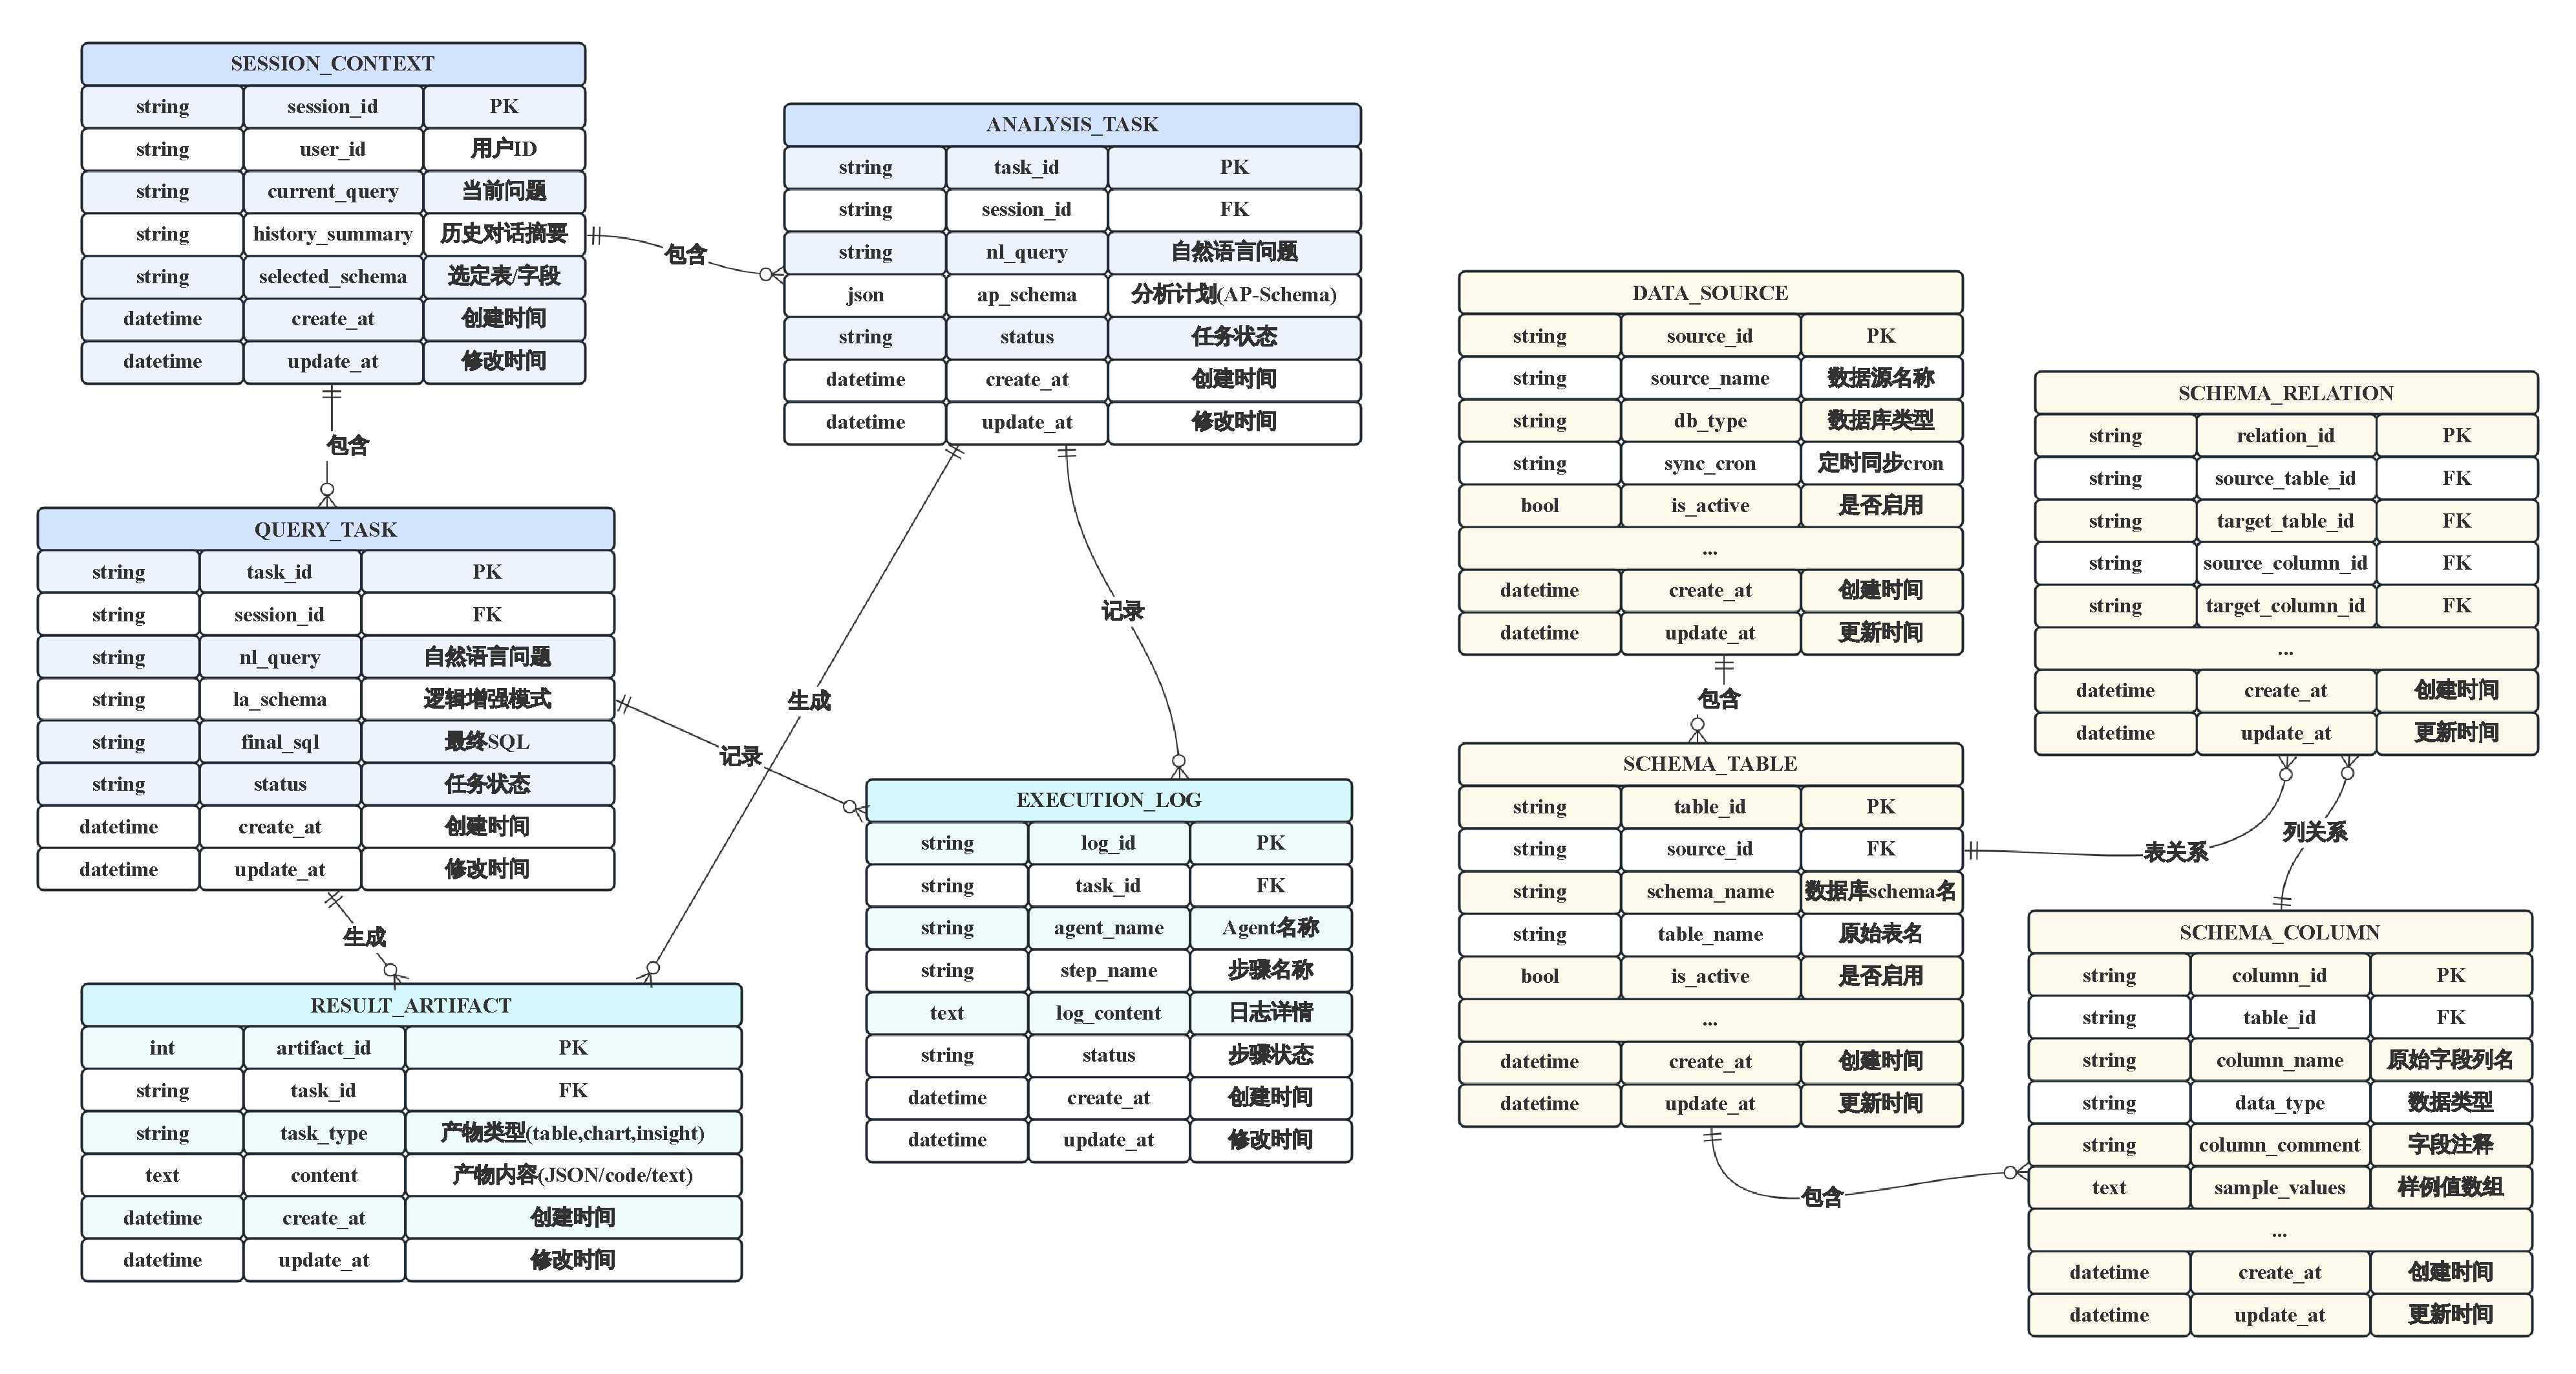
\includegraphics[width=1.0\textwidth]{figures/chap05/fig5-6_metadata_er.pdf}
	\caption{系统元数据库ER图}\label{fig:chap05_er}
\end{figure}

从结构关系看，源数据侧由\texttt{data\_source}和三类\texttt{schema\_*}元数据表共同构成统一结构描述；
会话侧由\texttt{session\_context}、\texttt{query\_task}和\texttt{analysis\_task}共同构成交互过程的状态管理；
产物侧则由\texttt{result\_artifact}和\texttt{execution\_log}承接任务级结果沉淀与运行留痕。
由于查询任务和分析任务都可能生成多个结果文件和多条日志记录，因此系统将产物和日志分别设计为独立从表，并通过\texttt{task\_type}与\texttt{task\_id}完成关联。

这一设计有两点工程收益。
其一，查询和分析虽然属于不同任务类型，但可以共享同一套产物管理与日志管理机制，从而减少重复设计；
其二，任何任务在结束后都能够通过任务ID回溯到对应的SQL、AP-Schema、结果文件和异常日志，从而支撑第五章强调的可追溯性要求。

\subsection{结果、日志与缓存管理}

在持久化存储策略上，系统并不将所有内容都塞入同一种存储引擎，而是根据对象类型分别落到最合适的组件中。
具体而言，PostgreSQL负责保存系统元数据、任务主记录和领域知识库；Milvus负责保存字段值向量和样例向量索引；Redis负责热点缓存；图表文件、导出文件和大体积结果文件则采用文件路径方式登记到\texttt{result\_artifact}中。
这种“结构化状态入库、检索索引入向量库、热点结果入缓存、文件产物入对象路径”的分层策略，与本研究的方法结构保持一致。

在\textbf{结果管理}方面，系统将查询结果表、图表文件、洞察文本、导出文件统一抽象为结果产物。
对于查询任务，重点保存\texttt{final\_sql}、结果表摘要和原始结果文件；对于分析任务，重点保存\texttt{ap\_schema}、图表描述、分析表格和\texttt{insights}文本。
若用户在已有查询结果基础上继续发起分析任务，系统可直接读取最近一次\texttt{result\_artifact}，减少重复计算。

在\textbf{日志管理}方面，\texttt{execution\_log}采用结构化写法，至少记录代理名称、执行步骤、输入摘要、状态、错误消息和时间戳。
与仅保存文本日志不同，结构化日志可以支持按任务、代理或步骤维度检索，使开发者能够快速定位错误是发生在模式链接、候选判别、分析算子还是结果封装环节。

在\textbf{缓存管理}方面，系统主要缓存两类内容。
第一类是变化频率较低但访问频繁的元数据与知识对象，如表结构摘要、字段样例值和部分领域知识片段；
第二类是高频相同请求对应的查询结果摘要或图表产物引用。
由于政务问数场景并不追求毫秒级实时更新，因此在保证缓存失效策略合理的前提下，引入Redis可以有效降低重复请求对数据库和大模型服务的压力。


\section{多智能体协同与上下文管理实现}

查询方法和分析方法都涉及多个推理步骤，如果将所有能力直接塞入单一长链路中，不仅工程实现复杂，而且流程可解释性和可控性都较弱。
为此，本文在智能服务层采用轻量级多智能体协同方式：并非追求通用自治智能体，而是通过明确的角色分工，将不同方法模块封装为职责清晰、接口稳定的服务角色。

\begin{figure}[htbp]
	\centering
	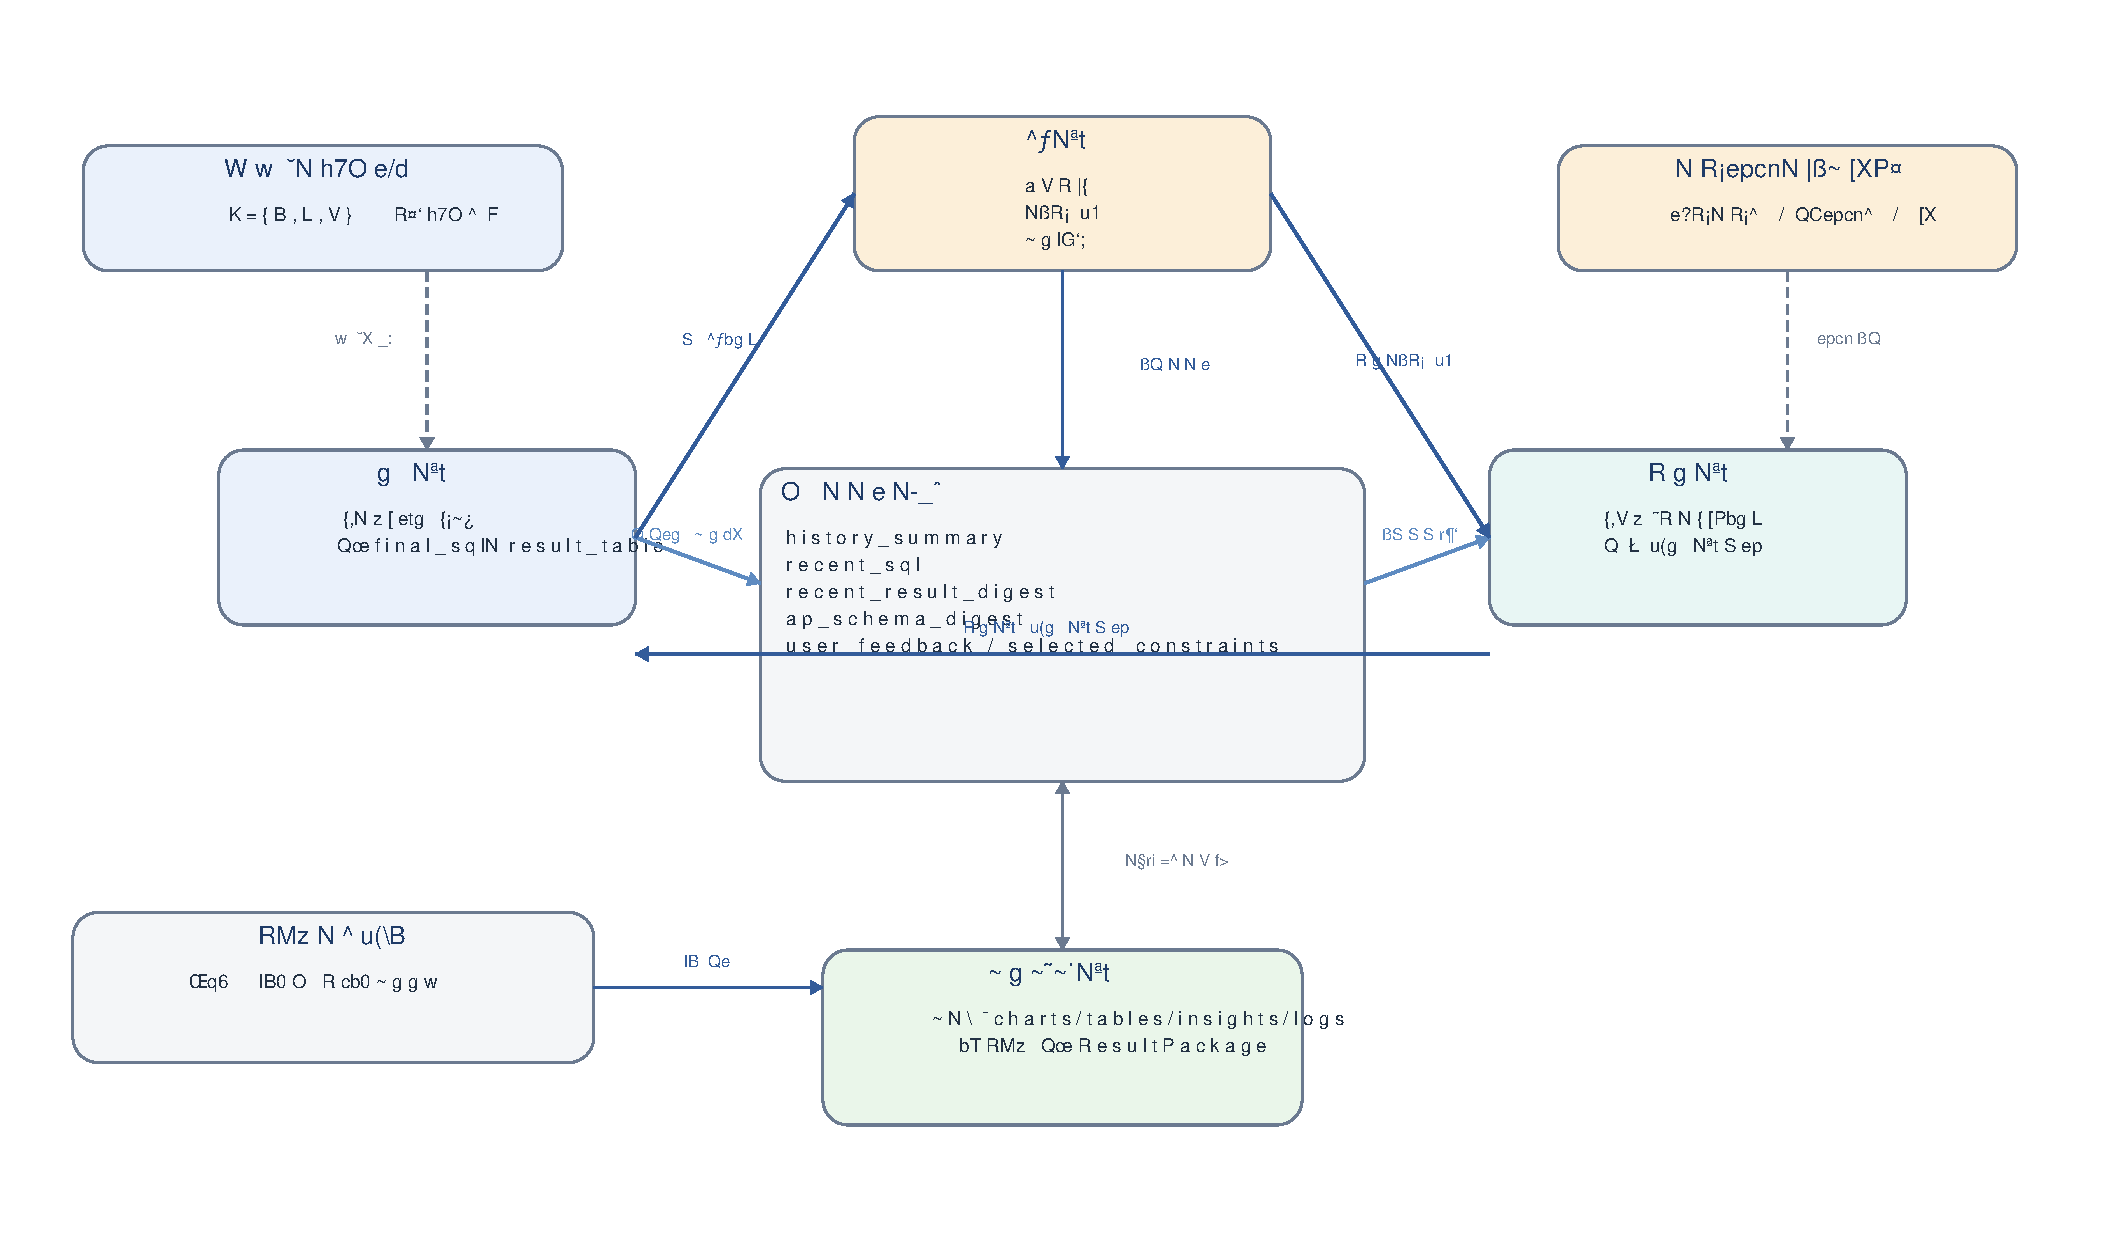
\includegraphics[width=0.95\textwidth]{figures/chap05/fig5-3_agent_context.pdf}
	\caption{轻量级多智能体协同与上下文传递图}\label{fig:chap05_agents}
\end{figure}

\subsection{轻量级多智能体角色设计}

如图\ref{fig:chap05_agents}所示，系统主要包含调度代理、查询代理、分析代理和结果组织代理四类角色。

\textbf{调度代理}是系统级入口角色。
它负责接收来自应用层的标准请求，判断当前任务属于查询还是分析，并根据会话状态决定是否需要附带历史上下文、最近结果产物或用户修正约束。
调度代理本身不负责生成SQL或执行分析，而是承担任务理解、路由和跨服务编排职责。

\textbf{查询代理}是“可靠取数专家”。
它完整封装第三章的方法，内部负责LA-Schema构建、异构候选生成、执行反馈修复和候选判别，对外部仅暴露稳定查询接口。
因此，无论任务来自用户的直接查询请求，还是来自分析代理的查询增强取数请求，最终都通过统一的查询代理执行。

\textbf{分析代理}是“分析规划与算子执行专家”。
它完整封装第四章的方法，负责从自然语言需求中生成AP-Schema，进行$Q_A/P_A$投影，并在查询结果返回后组织轻量分析算子链和可视化规则。
分析代理的专长在于规划和分析，而非从零生成数据库查询，因此它在取数阶段必须调用查询代理，而不是自行绕过查询服务。

\textbf{结果组织代理}位于系统输出端。
其核心任务并非额外推理，而是统一整合查询结果表、图表规格、图表文件、文字洞察和执行日志，输出供前端展示和元数据库登记的\texttt{ResultPackage}。
借助这一角色，查询服务和分析服务都不需要关心前端最终如何展示结果，从而保持职责边界清晰。

\subsection{查询与分析服务编排}

在多智能体框架下，最关键的设计不是角色数量，而是服务之间的调用关系是否稳定。
本系统中，查询服务和分析服务的对外接口被刻意设计为少字段、强约束的形式。

对于查询服务，其输入与输出接口进一步约束为：
\begin{quote}
\texttt{Input: nl\_query / session\_summary / optional\_constraints}\\
\texttt{Output: final\_sql / result\_table / execution\_status / logs}\\
\texttt{\hspace*{2.1em} / la\_schema\_snapshot}
\end{quote}
这意味着调度代理、分析代理甚至后续扩展模块都可以把查询代理视为“黑盒取数服务”，只要提供规范输入，就能得到稳定输出。

对于分析服务，其接口形态与之对应：
\begin{quote}
\texttt{Input: nl\_query / session\_summary / optional\_prior\_artifact}\\
\texttt{Output: ap\_schema / charts / tables / insights / logs}
\end{quote}
在这一接口中，\texttt{optional\_prior\_artifact}允许系统在“先查后析”的连续交互场景下复用已有结果，而\texttt{ap\_schema}和\texttt{logs}又保证了分析过程本身可查看、可复核。

从编排关系看，简单查询流程是线性的，即“调度代理 $\rightarrow$ 查询代理 $\rightarrow$ 结果组织代理”；
复杂分析流程则呈现为“调度代理 $\rightarrow$ 分析代理（规划）$\rightarrow$ 查询代理（取数）$\rightarrow$ 分析代理（算子执行）$\rightarrow$ 结果组织代理”的组合链路。
这种设计看似拉长了调用路径，但它把复杂任务拆解为稳定的服务节点，避免分析代理内部再次实现一套自由SQL生成逻辑，从而保持系统与第三章、第四章的方法边界一致。

\subsection{上下文维护与状态流转}

多轮问数、连续追问以及从查询平滑过渡到分析，是政务智能问数应用的重要交互特征。
因此，系统不能只保留“当前问题”这一单点输入，而需要维护一个能够支撑状态继承和上下文压缩的会话模型。

在本系统中，\texttt{session\_context}并不简单保存所有历史文本，而是重点维护五类必要状态：
\textbf{（1）历史问题摘要，}用于保留主题连续性；
\textbf{（2）最近一次成功查询的SQL摘要，}用于省略式追问；
\textbf{（3）最近一次结果表或分析产物摘要，}用于“在刚才数据基础上继续分析”；
\textbf{（4）AP-Schema摘要，}用于连续分析任务继承分析类型、粒度和展示偏好；
\textbf{（5）用户修正反馈与选定约束，}用于减少后续字段歧义和条件漂移。

基于这些状态，系统支持三类典型状态流转。
第一类是\textbf{上下文继承}：例如用户在查询“A区预算收入”后继续追问“那B区呢”，系统可在继承原问题指标与时间条件的前提下，仅替换筛选条件；
第二类是\textbf{上下文压缩}：随着会话轮数增加，系统不会无上限拼接全部历史，而是将较早内容压缩为摘要并保留最近几轮关键信息，兼顾信息完整性和大模型上下文长度限制；
第三类是\textbf{查询到分析的状态过渡}：当用户在一条查询结果之后继续发起趋势分析或结构分析时，分析代理可直接读取最近一次\texttt{result\_artifact}和其摘要，而不必重新理解完整的上游场景。

通过这种细粒度的上下文维护机制，系统得以将一次次独立请求组织成一条连续、可继承、可追溯的交互链路，这也是论文原型系统能够体现“智能问数”而非“单轮SQL生成”的关键实现支撑。


\section{系统功能实现与效果展示}

基于上述架构、流程和数据存储设计，论文原型系统在前端侧组织为四类核心页面，分别对应自然语言输入、SQL与结果查看、分析结果展示以及任务追溯查看。
由于本章采用的是论文原型口径，图\ref{fig:chap05_wireframe}使用页面线框图而非真实产品截图展示系统界面结构。

\begin{figure}[htbp]
	\centering
	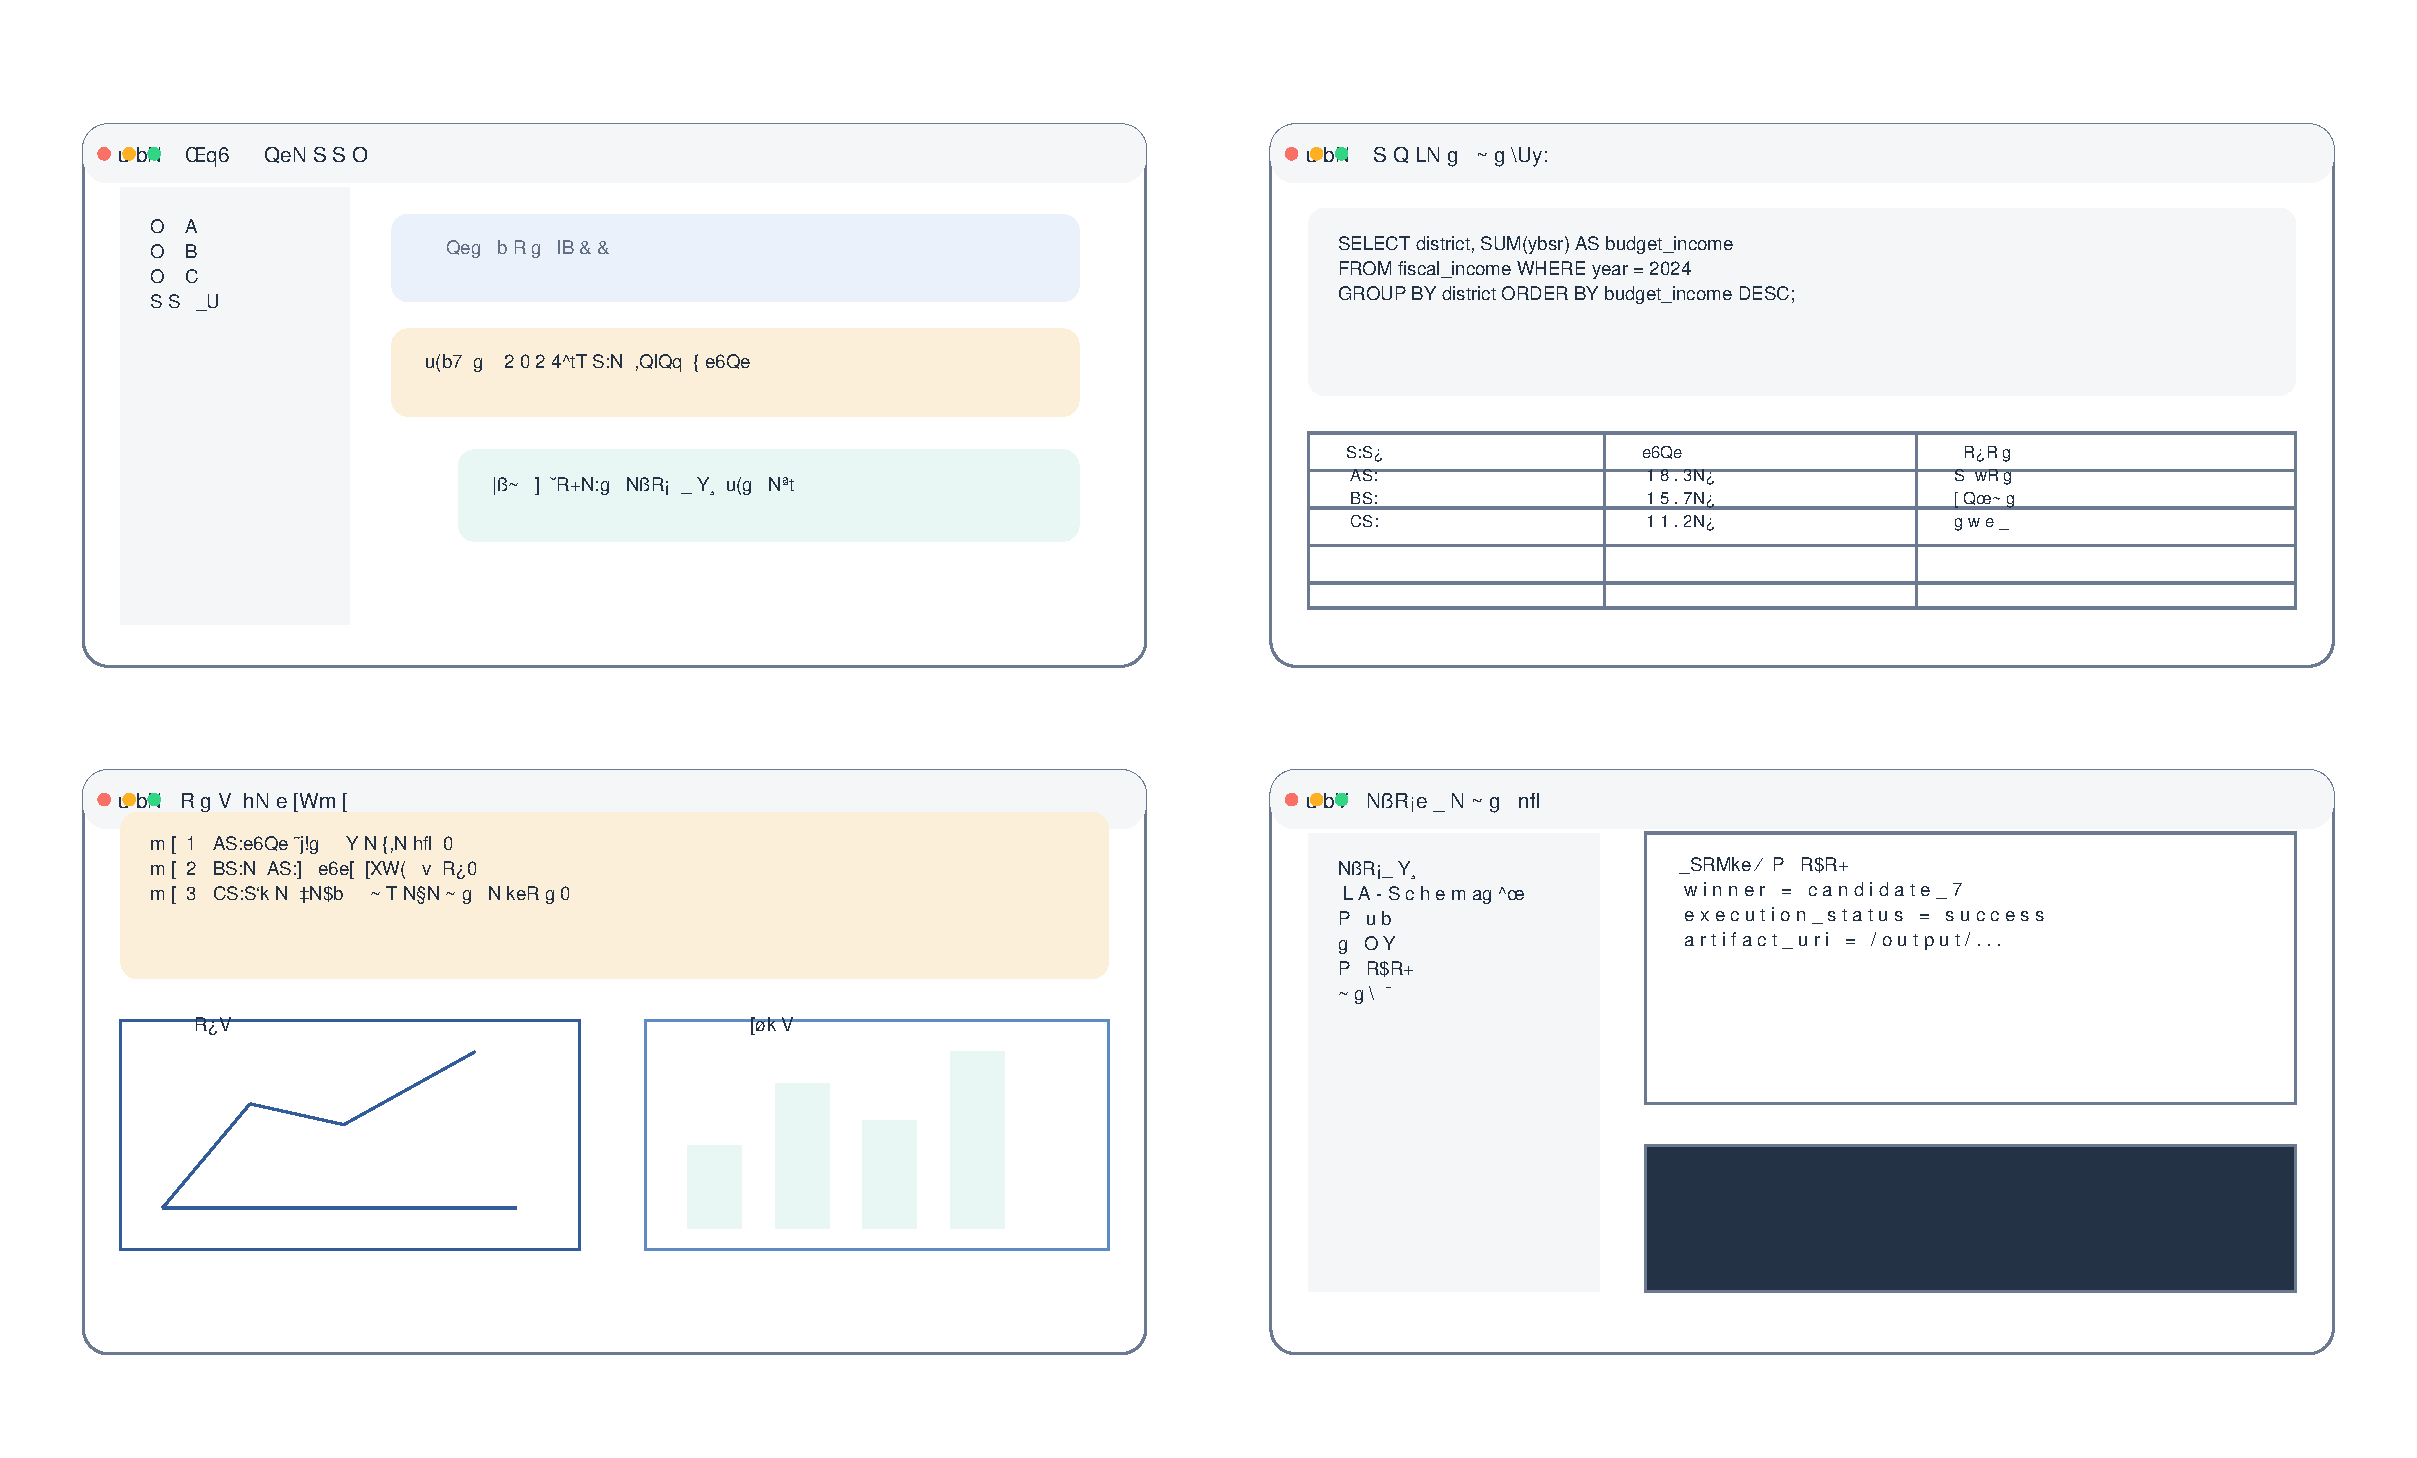
\includegraphics[width=1.0\textwidth]{figures/chap05/fig5-8_ui_wireframe.pdf}
	\caption{系统核心功能页面线框图}\label{fig:chap05_wireframe}
\end{figure}

\textbf{页面一：自然语言输入与历史会话页。}
该页面是系统的主要交互入口，顶部提供自然语言输入框，左侧提供历史会话列表，主区域展示用户与系统的交互内容。
用户可以直接输入查询类或分析类需求，也可以在已有会话中继续追问。
这一页面对应第五章的任务接入与上下文管理机制，是多轮问数的起点。

\textbf{页面二：SQL与查询结果展示页。}
当任务被判定为查询类请求并成功执行后，系统在该页面展示最终SQL语句和结果表。
其中，SQL区域提升系统透明度，便于用户理解“系统到底查了什么”；结果表区域则为后续人工复核、导出或发起一键分析提供基础。
这一页面对应第三章方法在原型系统中的直接工程体现。

\textbf{页面三：分析图表与文字洞察页。}
当任务属于分析类请求，或用户在查询结果基础上发起分析时，系统在该页面展示图表、分析表格和文字洞察。
其中，图表展示承接第四章的可视化规则与图表后校正逻辑，文字洞察承接第四章的摘要生成要求，分析表格则作为图表和结论的结构化支撑。
这一页面对应第四章方法在原型系统中的结果呈现形态。

\textbf{页面四：任务日志与结果追溯页。}
该页面用于查看任务执行路径、代理调用步骤、中间产物和最终结果文件，是系统可解释性和可追溯性的集中体现。
当用户需要了解为何某次查询失败、最终采用了哪条SQL、分析结果基于哪一份取数结果生成时，都可以在该页面中完成回溯。
这一页面与前文的\texttt{execution\_log}、\texttt{result\_artifact}和\texttt{session\_context}设计直接对应。

由此可见，系统功能页面并不是独立于方法之外的界面拼装，而是把第三章的查询能力、第四章的分析能力以及第五章的会话管理、结果追溯机制，通过统一交互界面组织到一个可用的原型系统中。
用户在界面层面看到的是一次自然的问数与分析过程，而在系统内部则对应着多代理协同、标准结果接口和结构化状态流转的工程实现。


\section{本章小结}

本章从工程实现角度，对面向政务场景的大模型数据查询与分析原型系统进行了系统化设计与说明。
与第三章和第四章侧重方法创新不同，本章的核心工作是将“可靠查询生成”和“规范分析生成”组织为一个可交互、可追溯、可扩展的统一原型系统。

具体而言，本文构建了由表示层、应用层、智能服务层和数据层组成的四层体系，并在智能服务层中设计了由调度代理、查询代理、分析代理和结果组织代理构成的轻量级多智能体协同框架。
在此基础上，系统实现了从自然语言请求进入、LA-Schema增强取数、AP-Schema规划分析、标准结果接口传递，到结果包封装和执行日志留痕的完整处理链路。
同时，围绕元数据抽取、系统元数据库、缓存和结果文件的存储设计，为多轮交互、结果复用和问题追溯提供了稳定支撑。

因此，本章不仅给出了第三章与第四章方法在工程层面的落地方式，也证明了“查询生成服务 + 分析生成服务 + 轻量级多代理编排 + 上下文管理”这一组合能够形成一个逻辑自洽的政务智能问数原型系统，为全文后续结论与应用价值论证提供了实现基础。
